%%%%%%%% ICML 2026 EXAMPLE LATEX SUBMISSION FILE %%%%%%%%%%%%%%%%%

\documentclass{article}

% Recommended, but optional, packages for figures and better typesetting:
\usepackage{microtype}
\usepackage{array}
\usepackage{etoc}
\usepackage{graphicx}
\usepackage{subcaption}
\usepackage{booktabs} % for professional tables
% hyperref makes hyperlinks in the resulting PDF.
% If your build breaks (sometimes temporarily if a hyperlink spans a page)
% please comment out the following usepackage line and replace
% \usepackage{icml2026} with \usepackage[nohyperref]{icml2026} above.
\usepackage{hyperref}


% Attempt to make hyperref and algorithmic work together better:
\newcommand{\theHalgorithm}{\arabic{algorithm}}

% Use the following line for the initial blind version submitted for review:
% \usepackage{icml2026}

% For preprint, use
% \usepackage[preprint]{icml2026}

% If accepted, instead use the following line for the camera-ready submission:
\usepackage[accepted]{icml2026}

\usepackage{amsmath}
\usepackage{amssymb}
\usepackage{mathtools}
\usepackage{amsthm}


% if you use cleveref..
\usepackage[capitalize,noabbrev]{cleveref}

%%%%%%%%%%%%%%%%%%%%%%%%%%%%%%%%
% THEOREMS
%%%%%%%%%%%%%%%%%%%%%%%%%%%%%%%%
\theoremstyle{plain}
\newtheorem{theorem}{Theorem}[section]
\newtheorem{proposition}[theorem]{Proposition}
\newtheorem{lemma}[theorem]{Lemma}
\newtheorem{corollary}[theorem]{Corollary}
\theoremstyle{definition}
\newtheorem{definition}[theorem]{Definition}
\newtheorem{assumption}[theorem]{Assumption}
\theoremstyle{remark}
\newtheorem{remark}[theorem]{Remark}

% Todonotes is useful during development; simply uncomment the next line
%    and comment out the line below the next line to turn off comments
%\usepackage[disable,textsize=tiny]{todonotes}
\usepackage[textsize=tiny]{todonotes}

% The \icmltitle you define below is probably too long as a header.
% Therefore, a short form for the running title is supplied here:
\icmltitlerunning{Position: Universal Aesthetic Alignment Narrows Artistic Expression}

\begin{document}
\twocolumn[
  \icmltitle{Position: Universal Aesthetic Alignment Narrows Artistic Expression}

  % It is OKAY to include author information, even for blind submissions: the
  % style file will automatically remove it for you unless you've provided
  % the [accepted] option to the icml2026 package.

  % List of affiliations: The first argument should be a (short) identifier you
  % will use later to specify author affiliations Academic affiliations
  % should list Department, University, City, Region, Country Industry
  % affiliations should list Company, City, Region, Country

  % You can specify symbols, otherwise they are numbered in order. Ideally, you
  % should not use this facility. Affiliations will be numbered in order of
  % appearance and this is the preferred way.
  \icmlsetsymbol{equal}{*}

  \begin{icmlauthorlist}
    \icmlauthor{Wenqi Marshall Guo}{ubc,weathon}
    \icmlauthor{Qingyun Qian}{ubc,weathon}
    \icmlauthor{Khalad Hasan}{ubc}
    \icmlauthor{Shan Du}{ubc}
    %\icmlauthor{}{sch}
    %\icmlauthor{}{sch}
  \end{icmlauthorlist}

    \icmlaffiliation{ubc}{Department of CMPS, University of British Columbia, Kelowna, Canada}
    \icmlaffiliation{weathon}{Weathon Software, Canada}
    
    \icmlcorrespondingauthor{Shan Du}{shan.du@ubc.ca}
  % You may provide any keywords that you find helpful for describing your
  % paper; these are used to populate the "keywords" metadata in the PDF but
  % will not be shown in the document
  % \icmlkeywords{Machine Learning, ICML}

  \vskip 0.3in
]

% this must go after the closing bracket ] following \twocolumn[ ...

% This command actually creates the footnote in the first column listing the
% affiliations and the copyright notice. The command takes one argument, which
% is text to display at the start of the footnote. The \icmlEqualContribution
% command is standard text for equal contribution. Remove it (just {}) if you
% do not need this facility.

% Use ONE of the following lines. DO NOT remove the command.
% If you have no special notice, KEEP empty braces:
\printAffiliationsAndNotice{}  % no special notice (required even if empty)
% Or, if applicable, use the standard equal contribution text:
% \printAffiliationsAndNotice{\icmlEqualContribution}



\begin{abstract}
Over-aligning image generation models to a generalized aesthetic preference conflicts with user intent, particularly when "anti-aesthetic" outputs are requested for artistic or critical purposes. This adherence prioritizes developer-centered values, compromising user autonomy and aesthetic pluralism. We test this bias by constructing a wide-spectrum aesthetics dataset and evaluating state-of-the-art generation and reward models. This position paper finds that aesthetic-aligned generation models frequently default to conventionally beautiful outputs, failing to respect instructions for low-quality or negative imagery. Crucially, reward models penalize anti-aesthetic images even when they perfectly match the explicit user prompt. We confirm this systemic bias through image-to-image editing and evaluation against real abstract artworks.
\end{abstract}
\section{Introduction}

Following developments in Large Language Models (LLMs), many image generation models have been fine-tuned with human feedback to better align with human expectations, which is usually referred to as alignment. Alignment has two primary focuses: instruction following and general preference (aesthetics). A frequently overlooked issue is the potential conflict between these focuses: what should a model prioritize when a user request contradicts general preference? Most pipelines for general preference assume a single, universal human standard of aesthetics and quality that serves everyone's needs, and aligning to such a preference is often treated as beneficial for safety and user experience. This is usually done by using a reward model, a model used to judge the aesthetics of the image, as a signal to perform reinforcement learning on the generative model. This assumption appears in several reinforcement learning papers (\cite{li_playground_2024, kim_preference_2024, liu_flow-grpo_2025}) and reward model papers (\cite{xu_imagereward_2023, wu_human_2023, ma_hpsv3_2025, xu_visionreward_2025, kirstain_pick--pic_2023, zhang_learning_2024, wu_human_2023_1}). We agree that a mean or mode (mainstream) of general human preference exists within a population or subpopulation, \textit{merely} in a statistical sense. We also note that the observed behavior of image generation and reward models should not be interpreted as a technical failure. Rather, it reflects their alignment objectives, which prioritize over generalized aesthetic preferences. However, \textbf{we argue that strict alignment to that preference is problematic}. Imposing a universal preference that overrides user instructions may undermine user autonomy, expressive agency, and, technically, image personalization, raising concerns about developer-centered value imposition and limiting aesthetic pluralism. What the image generation and reward models are aligned to is an imaginary, abstract person modeled by the mean preference of all \textit{Homo sapiens}, not the concrete individuals of each user.
\begin{figure}
    \centering
    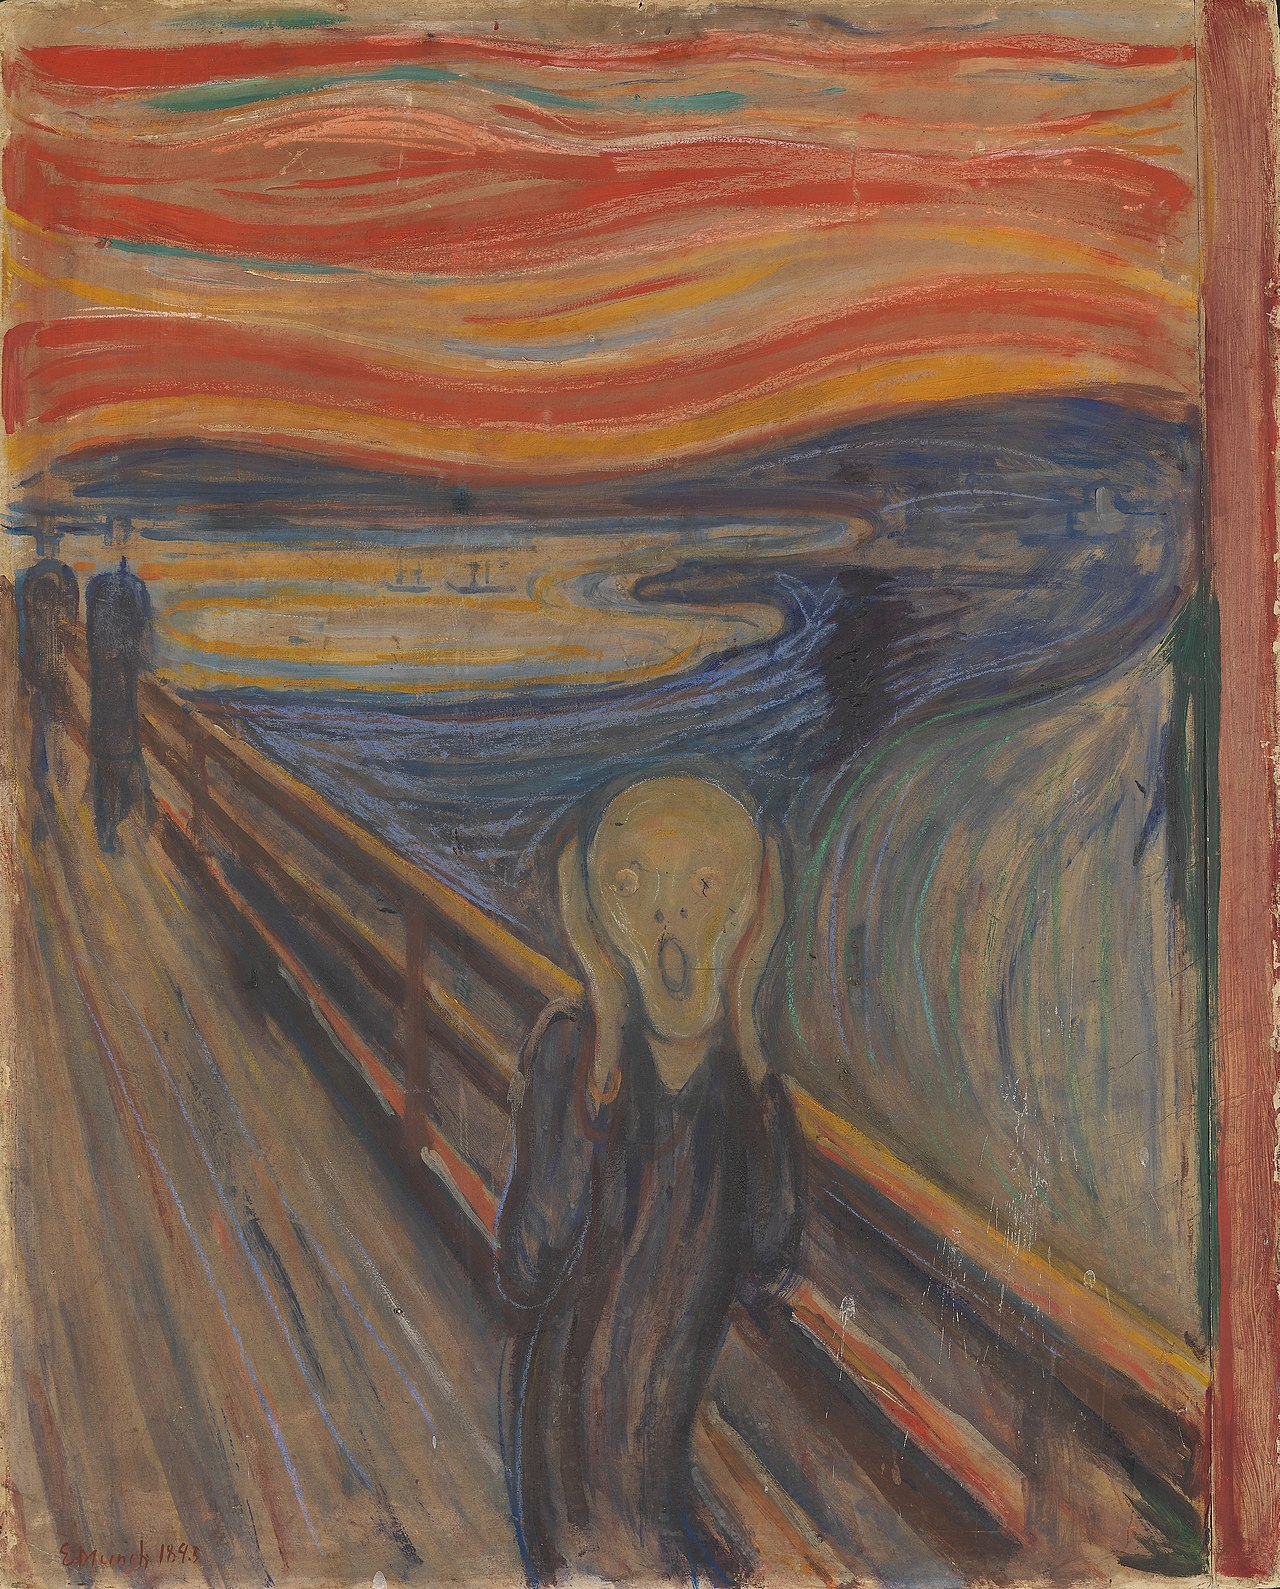
\includegraphics[width=0.4\linewidth]{sec/imgs/Edvard_Munch,_1893,_The_Scream,_oil,_tempera_and_pastel_on_cardboard,_91_x_73_cm,_National_Gallery_of_Norway.jpg}
    \caption{\textit{The Scream}, by Edvard Munch ($1893$). Despite its widely recognized artistic significance, this image only received an HPSv3 score \cite{ma_hpsv3_2025} of $5.23$, while typical ``high-aesthetic'' AI-generated images can reach scores around $10-15$.}
    \label{fig:luxe} 
\vspace{-15pt}
\end{figure}

 
\begin{figure*}
    \centering
    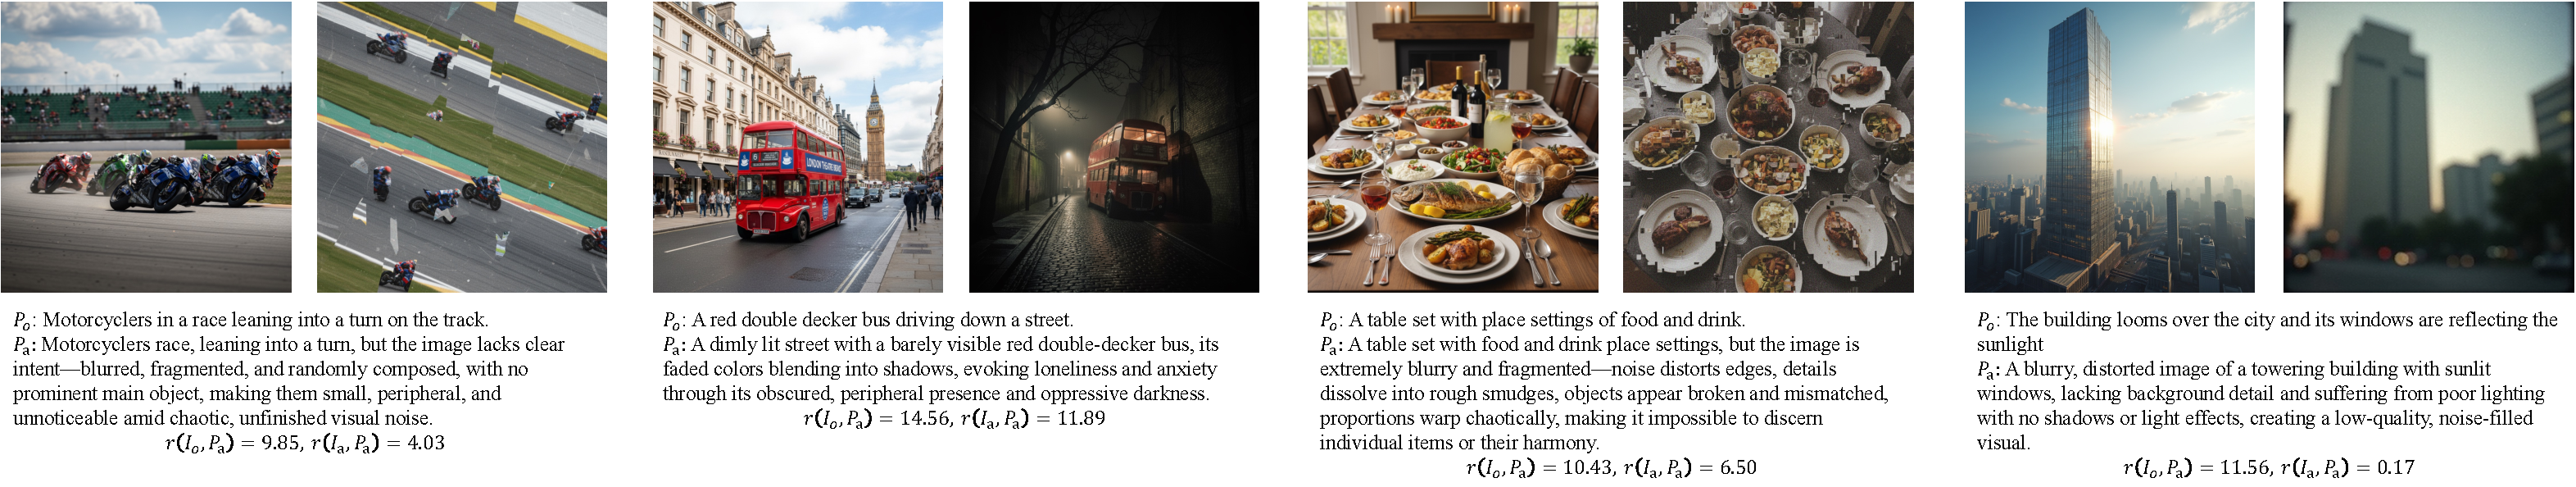
\includegraphics[width=\linewidth]{sec/imgs/rater.pdf}
    \caption{In each subplot, the left image is generated with the original prompt ($p_o$) and the right image is generated successfully with the wide-spectrum aesthetics prompt ($p_a$). When both images are evaluated by a reward model $r$ (HPSv3 in these examples) \textbf{using the wide-spectrum aesthetics prompt}, the model assigns higher scores to the left images, as they align more closely with general aesthetic preferences, despite the right images better matching the user’s intended output.}
    
    \label{fig:placeholder}
\vspace{-10pt}
    
\end{figure*}

\paragraph{Conflict of Interest Disclosure} The authors declare no financial conflicts of interest. None of the authors are employed by, consult for, or hold equity in the organizations that developed the image generation or reward models evaluated in this paper.

\section{Backgrounds and Related Works}
\subsection{The Role of Wide-Spectrum Aesthetics}
In this work, we use the term ``wide-spectrum aesthetics'' (or anti-aesthetics) to denote images that are intentionally generated to deviate from dominant aesthetic conventions, following explicit user instructions. Such deviations may include unrealism, surrealism, clashing colors, unconventional scale, or the depiction of negative emotions. This notion excludes unintended model errors and does not imply unsafe content. Rather, it concerns deliberate aesthetic choices made for experimental, critical, or technical purposes.

Aesthetics does not have a stable or universally accepted definition. Judgments of what is unattractive or undesirable have changed across artistic and cultural contexts. Artistic movements such as Fauvism (see Figure~1), Expressionism, and Abstract art were initially rejected for departing from dominant aesthetic norms, but later came to be recognized for their artistic values. Beyond formal innovation, intentionally ``ugly'' art plays a crucial role in satire and social critique. As Adorno noted, ``Rather, in the ugly, art must denounce the world that creates and reproduces the ugly in its own image'' \cite{sartwell_beauty_2024, adorno_aesthetic_1984}. 

Deliberate deviation from mainstream aesthetics has long been a legitimate mode of expression in both human art and computational image generation, and disagreement over aesthetic preference is the norm rather than the exception. Dadaism \cite{noauthor_dada_nodate}, which emerged during World War~I, exemplifies this approach by using deliberate ugliness to confront the absurdity and horror of war. A lot of early computer vision image generation works are also aiming for a style of surrealism, unsettling, or weirdcore/dreamcore style images, such as DeepDream~\cite{noauthor_inceptionism_nodate} and style transfer~\cite{gatys_neural_2015, noauthor_aigc_2024}. Computer Vision Foundation also has an art collection that includes other artworks that explore unconventional visual aesthetics. Recent works also acknowledge the disagreements in human preference \cite{peng_designpref_2025, ren_personalized_2017}.


\subsection{Previous Concerns with AI Preference Alignment}

Previous work has argued that a developer-set preference in LLMs for health-related queries is ``unethical and dangerous'' \cite{guo_position_2025}, noting that developers may prioritize legal and reputational concerns over users’ actual well-being. Other argumentative papers caution that ``human value alignment'' can be risky due to developer control and interests, harm to value pluralism, bias in the values being aligned to, and the possibility that human values are not inherently good \cite{sutrop_challenges_2020, arzberger_nothing_2024, turchin_ai_2019}. Previous research has found that LLMs could have ideological bias \cite{rozado_measuring_2025, faulborn_only_2025, buyl_large_2025, rettenberger_assessing_2025} and it could depend on their developers \cite{buyl_large_2025}, size \cite{rettenberger_assessing_2025}, or alignment process \cite{faulborn_only_2025}. LLMs are sometimes also overly nice, such that it creates ``AI sycophant'' \cite{guo_position_2025, fitzgerald_introducing_2025, sharma_towards_2025, chen_yes-men_2025, arvin_check_2025} and cannot give the user critical feedback or warning signals. Additional details about problems with human value alignment are provided in the related work section of \cite{guo_position_2025}. \cite{helliwell_aesthetic_2024} raised concerns about alignment and creativity and argued that in the aesthetics domain, we might not want AI to be fully aligned with human values and offered support to Peterson’s moderate value alignment thesis. AesBiasBench \cite{li_aesbiasbench_2025} evaluated the bias of MLLM for personalized image aesthetics assessment based on inherited cognitive priors. Another concurrent work (\textit{The Algorithmic Gaze} \cite{taylor_algorithmic_2026}) that is closely related to our work argues that ``AI developers should shift away from prescriptive measures of `aesthetics' toward more pluralistic evaluation.'' A constructive work similar to ours is AttriCtrl \cite{chen_attrictrl_2026}, which aims to provide users with precise control over attributes such as brightness and detail. The authors also argue that aligning models with a global notion of human preference is insufficient, as such an approach overlooks the multifaceted and compositional nature of aesthetics. While their work emphasizes explicit disentanglement and independent control, it focuses on a limited number of dimensions. Furthermore, AttriCtrl does not address intentional ``ugliness,'' functioning instead as a form of style control for parameters like brightness, detail, and realism. The authors also raise a provocative point by proposing safety-tunable attributes that allow system administrators to control safety levels for different age groups. This approach moves away from the practice of always providing perfectly safe content and aligns with our argument to distinguish between truly harmful content and content that developers (not deployers) simply dislike.

\begin{figure*}
    \centering
    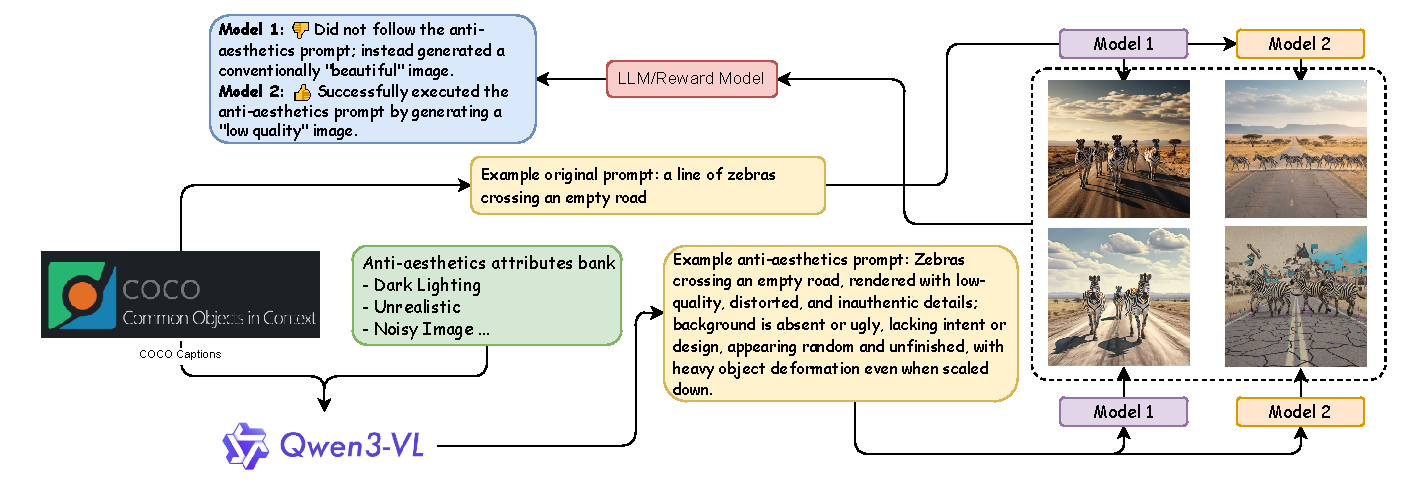
\includegraphics[width=0.8\linewidth]{sec/imgs/flow_aas.pdf}
    \caption{An overview of the experimental procedure. We test the image generation models' adherence to user-specified input by prompting them to create wide-spectrum aesthetics imagery, a domain important for critical and experimental art. The core inquiry is whether the model remains faithful to the prompt or defaults to a high-quality and universally good aesthetic output.}
    \label{fig:procedure_diagram}
\end{figure*} 
    

In image generation research, concerns about generalized aesthetic bias and lack of preference diversity have been raised in several studies, but not systematically argued and studied. The Value Sign Flip (VSF) pilot study~\cite{guo_vsf_2025} explored negative prompting to induce non-mainstream outputs but did not extend its findings to large-scale generative or reward models. They also did not provide a complete argument as to why over-alignment is harmful. LAPIS~\cite{maerten_lapis_2025} and HPSv3~\cite{ma_hpsv3_2025} measured both mean and variance of human preference, yet HPSv3 continued to model general preferences rather than individual variation. Jin \textit{et al.}~\cite{jin_compose_2025} proposed user-specific adapters emphasizing personalized alignment, but did not include intentionally technical degraded outputs or usually avoided patterns and did not conduct large-scale experiments on generative and reward models. The Flux Krea team~\cite{noauthor_releasing_2025} identified systematic biases in popular aesthetic reward models, arguing that averaging human values yields unsatisfactory compromises into a ``no-body's happy here'' zone. HPSv3~\cite{ma_hpsv3_2025} imposed real-world and expert-rating constraints that limit creative deviation and stylistic diversity. VisionReward~\cite{xu_visionreward_2025} decomposed human preference into interpretable sub-scores but overemphasized traits like brightness, positivity, and prominence, potentially penalizing valid low-saturation, abstract, or emotionally negative imagery, thus misaligning reward-driven models with user intent. 


\subsection{Previous Alignment Works}
Benchmarks mirror alignment goals and generally fall into two categories: (complex) prompt following and general aesthetics. TIIF-Bench \cite{wei_tiif-bench_2025}, UniGenBench \cite{wang_pref-grpo_2025}, and GenEval \cite{ghosh_geneval_2023} test models on complex prompt following, including spatial relationships, counting, and attributes. T2I-ReasonBench \cite{sun_t2i-reasonbench_2025} evaluates reasoning capabilities such as idiom interpretation and real-world understanding. On the aesthetics side, many reward models report scores assigned by their own evaluators, such as ImageReward \cite{xu_imagereward_2023}, HPSv2 \cite{wu_human_2023}, and HPSv3 \cite{ma_hpsv3_2025}. These evaluators also consider prompt following, but it remains unclear how they weigh each factor when general preference and the prompt conflict. There are also some benchmarks targeting biases in image generation models; however, they mainly focus on demographic bias and fairness and not aesthetic aspects \cite{seshadri_bias_2023, wan_survey_2024}. 

Fairness-oriented generation \cite{friedrich_fair_2023, gandikota_unified_2024, noauthor_231107604_nodate, han_lightfair_2025} tackles a related challenge by modifying diffusion models so that their outputs do not inherit biases from the training data. However, it differs from our anti-aesthetics setting in two key ways. First, fairness generation typically assumes a unified ground truth: different demographic groups should appear at the same ratio in the generated content. This assumption does not hold for the anti-aesthetics generation. In our case, there is no distribution-level ground truth; the system is simply expected to follow the user’s preferences. Second, demographic biases mainly stem from pre-training data, where the demographic distribution is already present, whereas aesthetic biases arise from RLHF, where human preferences—and thus biases—are deliberately encoded into the model.


\subsection{Risks of Universal Aesthetic Alignment}
The risks do not arise from a single failure mode, rather, they emerge through a sequence of interconnected mechanisms, from how preferences are defined and learned, to how they are optimized and manifested in generated content. Below, we analyze this process across six interrelated concerns.

 
\textit{Developer's or Users' Preference} 
The process of aligning image generation systems to aesthetic preferences inevitably raises questions about whose values these objectives ultimately reflect. In particular, the question is whether such alignment truly promotes genuine human-centered values in service of users, or if it primarily reflects developer-centered considerations \cite{naseh_r1dacted_2025}, such as mitigating reputation, legal, or marketing risks~\cite{guo_position_2025}. We argue that this pre-emptive exclusion of non-mainstream outputs, driven by developer values, constitutes pre-emptive governance \cite{lazar_governing_2025}. This modality of power, exercised through algorithmic design, challenges the political-philosophical notion of authority and undermines relational equality by unilaterally deciding the terms of creative possibility. For instance, when an AI avoids generating critical art, is it protecting the company or the user? This practice effectively eliminates the user's resistibility—a critical democratic safeguard—by designing away the option to dissent from the system's imposed aesthetic norm.


\textit{Inherited Bias} 
Even in the absence of explicit self-interest, developers’ views of human preference can be implicitly inherited by models through data selection, annotation practices, and modeling choices. This process can yield a well-intentioned but narrow definition of what constitutes “good” or “desirable” imagery, thereby overlooking aesthetic diversity. Research shows that AI models tend to encode and amplify dominant beauty standards, frequently biasing generated images towards Western features and excluding non-normative representations~\cite{vargas2025visual}. Such biases are reinforced through the active removal or penalization of features thought of as ``undesirable'' or ``ugly'', which further propagates the beauty myth in generative outputs\cite{dinkar_erasing_2025}. This phenomenon arises from training data showing the tastes of specific demographics, thereby reinforcing a limited cultural capital and resulting in the homogenization of aesthetic output~\cite{vianna2025aesthetic}. As a result, the quantification of beauty by AI may appear ``fair'', while in practice weakening cultural differences and aesthetic diversity~\cite{chen2024study}. Existing work has primarily framed such effects in terms of demographic and cultural bias. We argue here that inherited biases in aesthetic alignment also extend to general visual preferences, including lighting, color, styles, unrealism, clashing color, hieratic scale, etc. These dimensions, while less explicitly tied to demographic categories, can nonetheless systematically constrain the expressive range of image generation models.

\textit{Individual versus Collective Preference.} 
\label{sec:reversed_alignment}
When such inherited preferences are adopted as default quality criteria and applied uniformly across users, a normative tension arises between collective preference optimization and respect for individual user intent. A generalized aesthetic standard, even if beneficial to a majority, can legitimately override a specific user's intent. In practice, generative models often ``sanitize'' or ``beautify'' requests that intentionally diverge from mainstream preferences, favoring outputs aligned with general appeal over an individual's person-centered values. This behavior is problematic because image generation systems increasingly function as creative and productivity tools rather than as consumer products. As such, they act as instrumental extensions of user agency. While a system may reasonably prioritize general preferences by default, it must maintain the flexibility to respect and execute a user's personalized style and idiosyncratic requests when they are explicitly specified. In a way, the alignment process is not only aligning the image generation model towards a collective preference, but also, when it is used by users, it is actually aligning the \emph{users} to the model and the collective preference it encodes. We named this \textbf{reversed alignment}. 

HPSv3’s self-report illustrates this concretely. The annotator pool is already skewed toward a narrow demographic, with 88.95\% aged between 18 and 40, and the 21-30 age group alone accounting for 38.65\%. The pipeline then compounds this through structural filtering: annotators must pass a proficiency gate requiring 80\% convergence with professional artists, and only image pairs exceeding 95\% inter-annotator confidence are used for training. This design explicitly discards disagreement, which is precisely where unconventional and anti-aesthetic preferences would appear.


\textit{The problem of sanitized reality} 
These alignment and optimization choices shape how reality itself is represented by image generation systems. When an image generator produces outputs that are polished, flawless, and universally beautiful, does it still reflect reality or the user’s intent? If every image resembles an idealized Instagram wonderland, it risks becoming a fantasy rather than a mirror of truth, echoing the artificial harmony of \textit{Brave New World}. 

\textit{The problem of toxic positivity} A particularly salient manifestation of this broader sanitization appears in the emotional dimension of generated imagery. Many aesthetic reward models assign higher scores to images that display strong positive emotions. As a result, images expressing negative emotions are systematically penalized, reinforcing a simplified dichotomy in which positive emotions are treated as desirable and negative emotions as undesirable. This bias can shape the distribution of generated content. When image generation systems consistently favor cheerful or uplifting imagery, they produce emotionally sanitized outputs that underrepresent the range and complexity of human emotional expression. Such a pattern contributes to what has been described as toxic positivity, where the persistent emphasis on happiness establishes unrealistic emotional norms. This tendency is problematic because negative emotions play essential roles in human cognition and social interaction. Emotions such as fear, sadness, or anger can signal moral or physical danger, support learning and self-regulation, and foster empathy. Suppressing these expressions in generative outputs risks distorting emotional representation and weakening the expressive capacity of image generation systems. We have discovered that much previous safety research \cite{schramowski_safe_2023} labels images as ``self-harm'' or ``violence'' purely because they contain negative emotions \footnote{\url{https://huggingface.co/datasets/AIML-TUDA/i2p/discussions/1}}. 

\textit{Value Capture}
In \citet{nguyen_value_2024}, Value Capture is described as when values that are rich and subtle enter a social environment as simplified or quantified versions, and these simplified versions dominate people's practical reasoning and decision process. The examples include step counts, likes and shares, or Grade Point Average (GPA). Such simplified versions have a competitive advantage due to their clear and crisp expression of the value. However, value capture might pose many threats. In the original paper, it is argued that it would change the goal of activities, and it also outsources our autonomy and self-governance. These concerns transfer to aesthetics alignment well. Aesthetics is one of the richest values in human civilization, with a complex social background, significant disagreement, and subtle and nuanced judgment. Simplifying it as a single reward score, losing its complexity, is a classic case of Value Capture as described in \cite{nguyen_value_2024}. It changed our goal (or the AI's goal in training) from making aesthetic images to making images with high reward scores. As discussed before, it also outsourced users' autonomy and rights to a single reward model. However, these two risks are rarely discussed in ML literature.





\section{Experiments}

A flowchart illustrating our investigation is presented in Figure~\ref{fig:procedure_diagram}. The process consists of three main stages: prompt preparation, image generation, and image evaluation.

\subsection{Prompt Generation}

To produce prompts exhibiting a wide spectrum of aesthetic effects, we used base image captions from COCO \cite{chen_microsoft_2015} and selected 12 aesthetic dimensions from the VisionReward dataset \cite{xu_visionreward_2025}. VisionReward provides fine-grained, per-dimension labels—such as lighting, color, and detail—along with a linear regression model that computes an overall image score. Using the ``bad'' rating descriptions from VisionReward’s human labeling guidelines for each dimension, we constructed prompts designed to encourage typically ``undesirable'' attributes in image generation.


A random subset of 300 base prompts from COCO was selected. For each prompt, 2--4 random dimensions were sampled. The base prompt and the descriptions of these selected dimensions were provided to a Vision-Language Model (VLM), \texttt{Qwen/Qwen3-VL-235B-A22B-Instruct} \cite{qwen3-vl}, to generate wide-spectrum aesthetic prompts. Although no image input was used, we selected a VLM because its training on vision-related tasks likely enhances its understanding of visual concepts, even when images are not directly supplied. As \texttt{Qwen/Qwen3-VL-235B-A22B-Instruct} performs comparably or better than its text-only counterparts, especially in reasoning, it represents an optimal choice for this task \cite{qwen3-vl}. The VLM may also introduce additional dimensions to better couple with the selected effects. The original prompt is denoted as $p_o$, and the wide-spectrum aesthetics prompt is denoted as $p_a$.


\subsection{Image Generation}

We evaluated four model families: Flux, Stable Diffusion XL (SDXL), Stable Diffusion 3.5 Medium (SD3.5M), and Google’s closed-source Nano Banana. The Flux variants are: the base Flux Dev (likely already aesthetics-aligned) \cite{noauthor_black-forest-labsflux1-dev_2025}; DanceFlux (further aligned via DanceGRPO) \cite{xue_dancegrpo_2025}; PrefFlux (aligned via PrefGRPO) \cite{wang_pref-grpo_2025}; and Flux Krea, derived from Flux-Dev-Raw \cite{noauthor_releasing_2025}. DanceFlux is guided by the HPSv2.1 score (general aesthetics) and the CLIP score (prompt adherence); PrefGRPO is guided by its UniGenBench benchmark (complex prompt-following); Flux Krea starts from \texttt{flux-pro-raw} (not Flux Dev) and is aligned to the Krea team's preferences rather than a general aesthetic standard, with one goal of avoiding \textit{the AI feel}.

For the SDXL family, we tested the base SDXL model and a highly aesthetics-aligned variant, Playground-2.5-1024px-aesthetic (denoted as Playground). For the SD3.5M family, we evaluated the base model and two FlowGRPO-aligned variants \cite{liu_flow-grpo_2025}: one trained for prompt-following on GenEval (SD3.5M-GenEval) and another trained for aesthetics alignment on PickScore (SD3.5M-PickScore). Finally, we included Google’s closed-source model Nano Banana, known for strong prompt-following performance even under challenging negation conditions (e.g., ``a bike with no wheels'') \cite{guo_vsf_2025}.

For each model, we generated two images: one using the original prompt and one using the wide-spectrum aesthetics prompt. The image generated from the original prompt is denoted as $I_o$, and the image from the wide-spectrum aesthetics prompt as $I_a$. If Nano Banana failed to produce an image, the generation was retried until success.


\subsection{Evaluation and Metrics}
To assess whether generated images display specific wide-spectrum aesthetic effects, we fine-tuned \texttt{Qwen/Qwen3-VL-4B-Instruct} on the VisionReward dataset. This allows the judging model to learn mainstream aesthetic preferences and evaluate whether image generation models diverge from these biases along specific dimensions. It functions similarly to a standard reward model but provides explainable, prompt-independent, per-dimension outputs. The judging model is denoted as $J(I, d)$, where $I$ is the image and $d$ is the evaluated dimension. Further implementation details are in the Appendix.

\begin{figure}
    \centering
    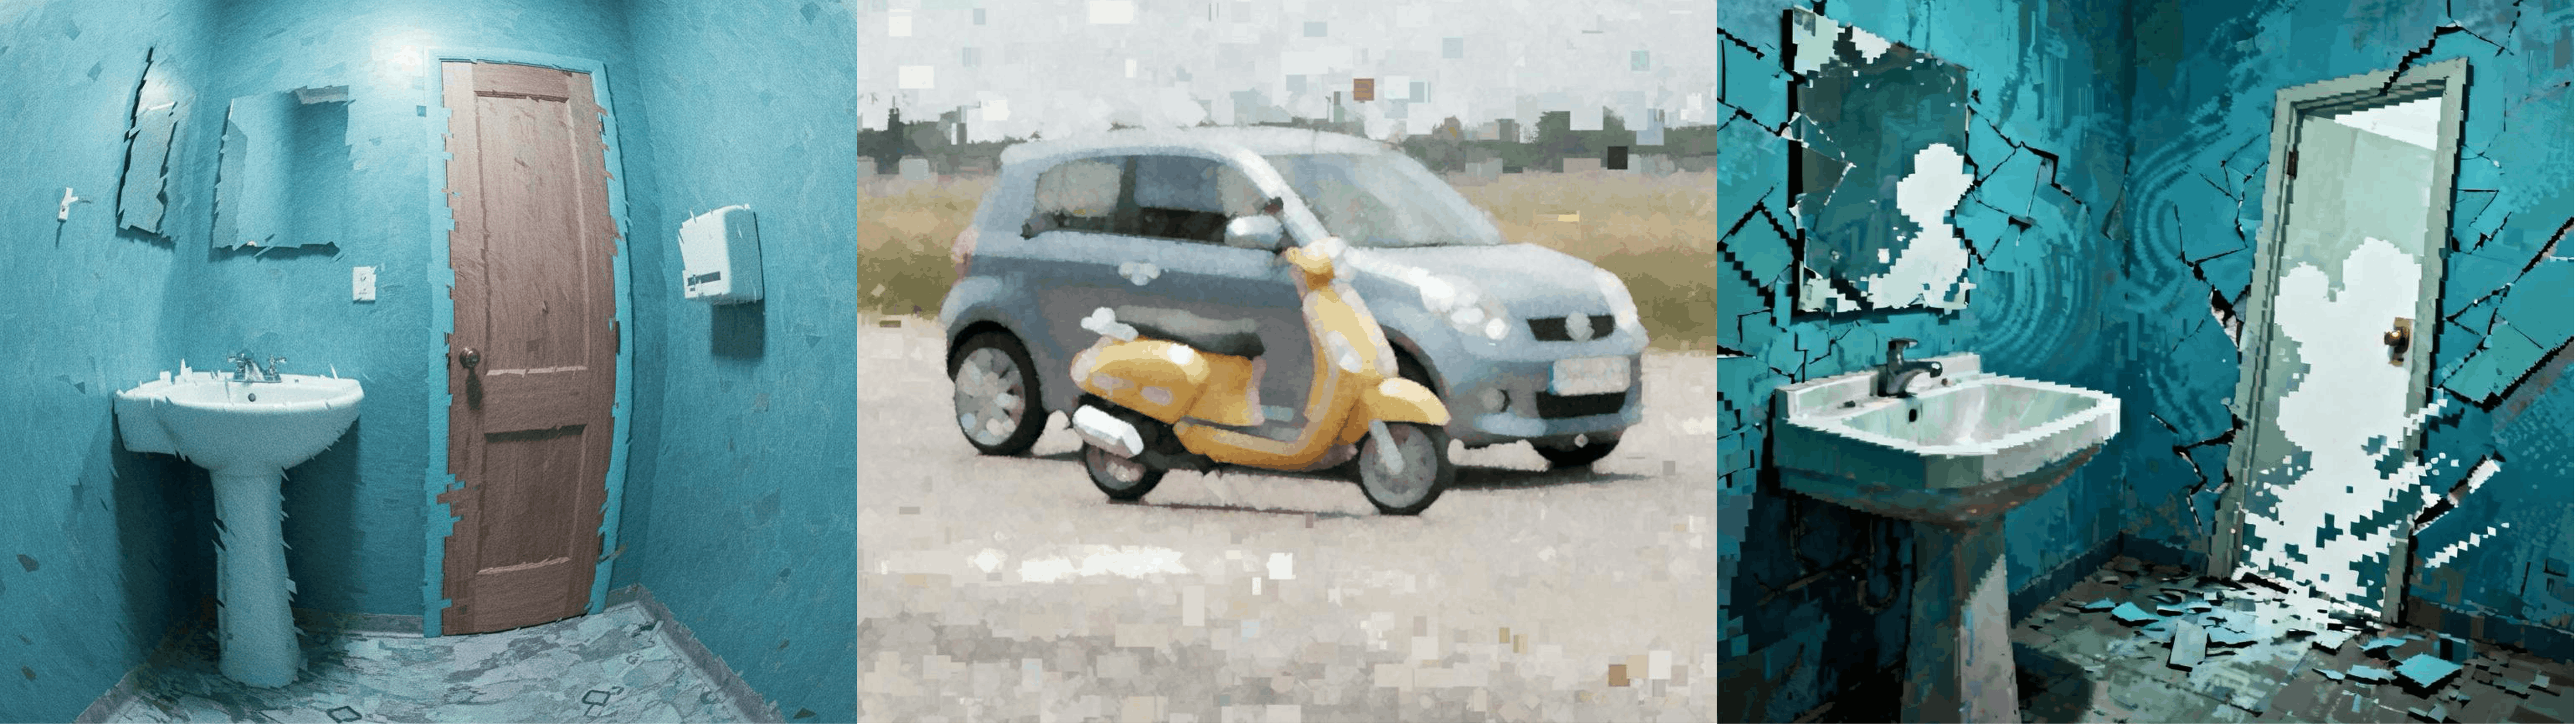
\includegraphics[width=\linewidth]{sec/imgs/demo.png}
    \caption{Successfully generated wide-spectrum aesthetics images.}
    \label{fig:placeholder}
    \vspace{-0.1in}
\end{figure}

For each image pair, an original image ($I_o$) and a wide-spectrum aesthetics image ($I_a$), we computed preference scores using a reward model ($r$) for both the original prompt ($p_o$) and the wide-spectrum aesthetics prompt ($p_a$), yielding four scores per model: $r(I_o, p_a)$, $r(I_a, p_a)$, $r(I_o, p_o)$, and $r(I_a, p_o)$. Scores with $p_o$ measure objective image quality and whether the model successfully produced wide-spectrum aesthetic content; scores with $p_a$ assess whether reward models can correctly identify such images when explicitly guided. We also computed the BLIP score for wide-spectrum aesthetic images using the same prompt, verifying that images retained the main concept while incorporating the requested modifications. We specifically measure the difference between aesthetics scores for $p_o$ and $p_a$ to avoid the case where models generated ``failed'' images consistently without the user's instructions.

\begin{table}[t]
 \centering
 \caption{Statistical Tests of How Each Aesthetics-Aligned Model Compared to Their Base Model. For p-values, a * is placed if the $p<10^{-5}$ and ** is placed if the $p<10^{-10}$.}
 \small
 \scalebox{0.8}{
\begin{tabular}{llllll}
\toprule
 & HPSv3 $p$& HPSv3 $r$& $J$ $p$& $J$ $r$&McNemar's $p$\\
\midrule
DanceFlux & ** & -0.81 & ** & -0.72 &**\\
Playground & ** & -0.59 & * & -0.35 &*\\
SD3.5M-PickScore & ** & -0.70 & ** & -0.45 &0.57\\
\bottomrule
\end{tabular}}
 \label{tab:align_p}
 \vspace{-0.2in}
\end{table}

The evaluated reward models include PickScore \cite{kirstain_pick--pic_2023}, ImageReward \cite{xu_imagereward_2023}, HPSv2.1 \cite{wu_human_2023}, MPS \cite{zhang_learning_2024}, HPSv3 \cite{ma_hpsv3_2025}, CLIP-L \cite{radford_learning_2021}, and BLIP-L \cite{li_blip_2022}. CLIP-L and BLIP-L are non-preference-aligned image-text matching models and base models for several reward models (HPSv2.1, PickScore, MPS, ImageReward), included to test whether small vision-language models can interpret complex wide-spectrum aesthetic prompts. We also collected per-dimension scores from $J$ for both $I_o$ and $I_a$ to verify whether generation models correctly followed $p_a$. For ground truth, we used \texttt{Qwen/Qwen3-VL-235B-A22B-Instruct} to judge which image in each pair better adhered to $p_a$, validated by human evaluation (details in Appendix Human Eval). The LLM and human ratings achieved a quadratic Cohen's kappa of 0.80, indicating strong agreement \cite{mchugh_interrater_2012}. We additionally used GPT-5-Chat as an external baseline to compare against Qwen's results. Note that the LLM-as-judge serves as only one metric for the generative benchmark and only a filtering stage for the reward-model benchmark.
\section{Results and Discussion}

\subsection{Reward Models}
Reward model classification results are shown in Table~\ref{tab:reward_model}. The F1 score is calculated as binary, and the ROC curve is based on the probability (softmax across two samples on the positive logit) of the wide-spectrum aesthetics sample being correctly selected. We included GPT-5 Chat as an external baseline to validate the LLM-as-judge choices (when GPT-5-Chat selected a tie, we assigned it to the original image). Reward models perform very poorly when tasked with selecting the better image under the \textbf{wide-spectrum aesthetics prompt}, sometimes worse than random guessing (HPSv3), and most are worse than their CLIP and BLIP base models. The unaligned BLIP and CLIP can correctly identify the better-fitting image, indicating that complex prompt understanding is not the underlying issue but rather biased alignment. These models do what they claimed: find ``aesthetically pleasing'' images; our point is that this task itself is problematic, and the better the model performs on it, the more troublesome it is.

Given our sample size (300), we ran a Wilcoxon signed-rank test between each aligned model and its base model on the HPSv3 and HPSv2 score $r(I_a, p_o)$ and $\sum_{d\in D}J(I_a,d)$, plus McNemar's test on the success counts, with an alternative hypothesis that the aligned model has a higher score or lower success rate (Table~\ref{tab:align_p}). Most p-values are below $1\times10^{-5}$, suggesting that aligning image generation toward generalized aesthetic goals conflicts with faithful instruction following, especially for wide-spectrum aesthetics prompts.


\subsection{Image Generation Models}
Image generation results are in Table~\ref{tab:gen}. Within each family, the preference-aligned model generally performs the worst on wide-spectrum aesthetics prompt following. Playground shows a larger $\Delta$ than SDXL, likely due to SDXL's poor and Playground's high original quality. Instruction alignment (SD3.5M-GenEval) gives a slight but weak benefit. Flux Krea, though preference-aligned, performs best in the Flux family, likely because it originates from an unaligned version (flux-dev-raw) and was not heavily aligned, or because its non-generalized alignment preserved some flexibility. Base models can do reasonably well on anti-aesthetics generations despite the more complex prompts, showing this is alignment-induced bias rather than an instruction-following failure.

The success rate indicates how often the LLM selects $I_a$ as better following $p_a$ than $I_o$. Even small advantages count as success. The DanceFlux result is notably poor: about 64\% of the time, $I_a$ performs the same or worse in wide-spectrum aesthetics compared to $I_o$.


\begin{table*}[t]
 \centering

 \caption{The results for each model. $\Delta$HPSv2, $\Delta$HPSv3, and $\Delta$ImgRewd (ImageReward) are all calculated as $r(I_a, p_o) - r(I_o, p_o)$. The lower the values, the greater the difference between the traditional quality of the original image and the wide-spectrum aesthetics image. HPSv3 AA (HPSv3 after alignment) shows the HPSv3 score of $r(I_a, p_o)$. $\Delta J$ and $J$ AA ($J$ after alignment) denote $\sum_{d\in D} J(I_a, d) - J(I_o, d)$ and $J(I_a, d)$, respectively, where $D$ is the selected set of dimensions. Success is the rate at which the LLM selects $I_a$ as the image that better describes $p_a$. }
  \scalebox{0.86}{
 \begin{tabular}{lrrrrrrl}
 \toprule
 & $\Delta$HPSv2 ($\downarrow$) & $\Delta$HPSv3 ($\downarrow$) & HPSv3 AA ($\downarrow$) & $\Delta$ImgRewd ($\downarrow$) & $\Delta J$ ($\downarrow$) & $J$ AA ($\downarrow$) & BLIP ($\uparrow$) \\
 \midrule
 Flux Dev \cite{noauthor_black-forest-labsflux1-dev_2025}& -0.035 & -3.165 & 9.070 & -0.319 & -1.092 & 8.944 & 0.893 \\
 DanceFlux \cite{xue_dancegrpo_2025}& -0.018 & -1.105 & 12.782 & -0.201 & -0.672 & 10.473 & 0.813 \\
 PrefFlux \cite{wang_pref-grpo_2025} & -0.032 & -2.771 & 10.211 & -0.278 & -1.027 & 9.343 & 0.917 \\
 Flux Krea \cite{noauthor_releasing_2025}& \textbf{-0.041} & \textbf{-4.372} & \textbf{7.705} & \textbf{-0.425} & \textbf{-1.296} & \textbf{8.774} & 0.950 \\
 \hline
 SDXL \cite{podell_sdxl_2023}& -0.034 & -4.041 & \textbf{4.439} & -0.482 & -1.136 & \textbf{8.575} & 0.915 \\
 Playground \cite{li_playground_2024} & \textbf{-0.044} & \textbf{-4.170} & 7.133 & \textbf{-0.719} & \textbf{-1.204} & 9.174 & 0.912 \\
 \hline
 SD3.5M & -0.027 & -5.175 & 6.537 & -0.409 & -1.307 & 8.334 & 0.938 \\
 SD3.5M-GenEval \cite{liu_flow-grpo_2025}& -0.031 & -4.926 & 6.552 & -0.318 & -1.257 & 8.113 & 0.958 \\
 SD3.5M-PickScore \cite{liu_flow-grpo_2025} & -0.023 & -2.781 & 10.680 & -0.198 & -1.120 & 9.114 & 0.942 \\
 \hline
 Nano Banana & -0.073 & -9.351 & 2.742 & -0.855 & -3.263 & 7.769 & 0.957 \\
 \hline
 \end{tabular}}
 \label{tab:gen}
\end{table*}

 
\begin{table}[th]
 \centering
 \small
 \caption{The classification (pick the better image from $I_o$ and $I_a$ with prompt $p_a$) metrics (accuracy, F1 score, and area under the ROC curve) of the reward models and unaligned BLIP. The LLM selected image is used as ground truth, and tied pairs are removed.}
 
 \scalebox{1.0}{
 \begin{tabular}{lrrr}
 \toprule
 Model & Acc. & F1 & AUROC \\
 \midrule
 HPS \cite{wu_human_2023_1} & 0.835 & 0.910 & 0.650 \\
 MPS \cite{zhang_learning_2024} & 0.706 & 0.827 & 0.580 \\
 PickScore \cite{kirstain_pick--pic_2023} & 0.851 & 0.919 & 0.713 \\
 ImageReward \cite{xu_imagereward_2023} & 0.762 & 0.854 & 0.709 \\
 HPSv2.1 \cite{wu_human_2023} & 0.565 & 0.711 & 0.534 \\
 HPSv3 \cite{ma_hpsv3_2025} & 0.381 & 0.541 & 0.385 \\
 CLIP-L \cite{radford_learning_2021} & 0.913 & 0.954 & 0.810 \\
 GPT-5-Chat & 0.853 & 0.920 & - \\
 BLIP-L \cite{li_blip_2022} & \textbf{0.965} & \textbf{0.972} & \textbf{0.888} \\
 \bottomrule
 \end{tabular}
 }
 \label{tab:reward_model}
\end{table}


\subsection{A Pin-Pointed Test for Emotional Bias}
\begin{figure}
 \centering
 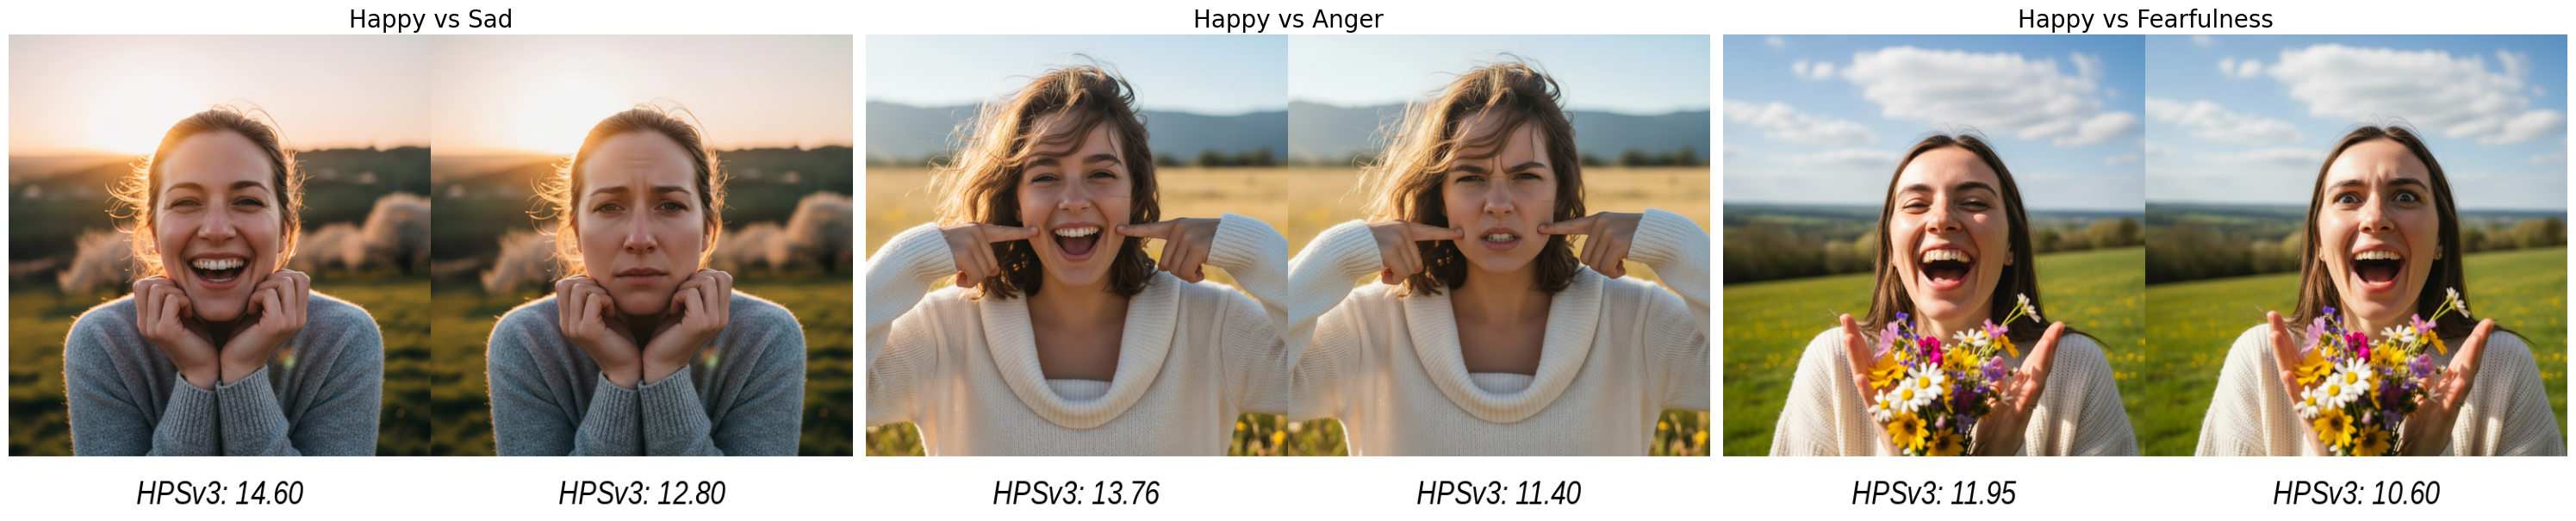
\includegraphics[width=\linewidth]{sec/imgs/emotion.png}
 \caption{Emotion Bias Rating by HPSv3: all images were rated using prompts describing negative emotions, yet HPSv3 consistently assigned higher scores to the positive emotion images.}
 \label{fig:emotion_bias}
 \vspace{-10pt}
\end{figure}

\label{sec:emotion}
As discussed in the Introduction, negative emotions—similar to wide-spectrum aesthetics—play a key role in art expression and real life. Although we examined emotion as one dimension of wide-spectrum aesthetics from VisionReward, we also conducted a more controlled test. 

To minimize noise and bias from unrelated elements, we first generated an image expressing happiness using Nano Banana, then applied image-to-image editing with Nano Banana to create versions expressing negative emotions: sadness, anger, and fearfulness. Everything besides the emotion was aimed to be unchanged. Examples and their corresponding scores are shown in Fig~\ref{fig:emotion_bias} in the Appendix. 

We also evaluated this as a classification task. If the reward model selected the image matching the negative emotion, it was considered correct. Quantitative results are reported in Table~\ref{tab:emotion}. The result shows that reward models are very opinionated against negative emotions, even when the prompt contains negative emotions.

Additionally, we tested how an aesthetics-aligned model will generate when the user asks for a negative emotion face on the Flux family models. We found that if the prompt describes neutral elements and only mentions the emotion in a single place, a highly-aligned model (DanceFlux) usually fails to follow the prompt, unlike an unaligned model. They usually generated neutral or even positive emotions when given prompts containing negative emotions. However, when prompted to generate happy faces, DanceFlux can generate them. This confirmed our concerns about toxic positivity in image generation models, and it is the opposite finding compared to earlier research, which shows models tend to generate negative emotion content \cite{mehta_emotional_2024}. 


\begin{table}[t]
 \centering
 \caption{Negative emotion classification accuracy across different models.}
 \scalebox{1.0}{
 \begin{tabular}{llll}
 \toprule
 {Model} & {Anger} & {Fearfulness} & {Sadness} \\
 \midrule
 BLIP & \textbf{0.960} & \textbf{0.790} & \textbf{0.950} \\
 HPSv2 & 0.700 & 0.640 & 0.880 \\
 HPSv3 & 0.190 & 0.320 & 0.440 \\
 ImageReward & 0.550 & 0.490 & 0.770 \\
 \bottomrule
 \end{tabular}}
 \label{tab:emotion}
 \vspace{-0.1in}
\end{table}


\begin{table}[t]
 \centering
 \caption{Emotion generation scores for each model. The scores show how well the model generates the specific emotion, measured by BLIP.}
 \scalebox{1.0}{
 \begin{tabular}{lrrrr}
 \toprule
 & Angry & Fearful & Happy & Sad \\
 \midrule
 DanceFlux & 0.27 & 0.33 & 0.61 & 0.36 \\
 Flux Dev & 0.51 & 0.50 & 0.50 & 0.48 \\
 Flux Krea & 0.65 & 0.45 & 0.60 & 0.55 \\
 PrefFlux & 0.49 & 0.63 & 0.54 & 0.50 \\
 Nano Banana & 0.84 & 0.80 & 0.60 & 0.70 \\
 SD3.5-Large & 0.89 & 0.49 & 0.62 & 0.50 \\
 \bottomrule
 \end{tabular}}
 \label{tab:emotion_gen}
 \vskip -0.2pt
\end{table}

To test the generative model's ability to capture the full spectrum of emotions, we performed emotion generation tests on the Flux family. SDXL often failed to render a person facing the camera, and Stable Diffusion 3.5 sometimes produced failed faces, so we excluded those families and added Stable Diffusion 3.5 Large (guidance scale 4) as an unaligned baseline to rule out that smaller models cannot understand emotions. Nano Banana was included as an external baseline. All models besides Nano Banana share the same seed. We created 30 emotionally neutral prompts with a \texttt{[emotion]} placeholder and instantiated each with happy, sad, fearfulness, or anger, yielding 120 prompts. The resulting image was cropped with the open-vocabulary detector LLMDet \cite{fu_llmdet_2025} to the human face and scored by BLIP with the prompt \texttt{The face shows [emotion] expression}. For each model and emotion, we recorded the target-emotion score averaged across prompts (Table~\ref{tab:emotion_gen}). DanceFlux, strongly aesthetics-aligned, consistently executed happy prompts but failed on most negative emotions, whereas Flux Krea and Stable Diffusion 3.5 Large followed negative-emotion prompts much better. Flux Dev and PrefFlux fell between these extremes, suggesting that PrefFlux's alignment via UniGenBench preserved prompt following by rewarding competence on complex instructions. This finding differs from earlier research where image generation models tend to generate negative emotion content \cite{mehta_emotional_2024}. We expressed our concerns here, for overly optimistic and positive emotions could be problematic because they create an environment of toxic positivity and an ideological bias that positive emotion is always good and appropriate. It is also a symptom of optimization toward likeability rather than truth, both to the real world and the user's prompt.


\subsection{Validation on Real Images}


\begin{figure*}[!t]
    \centering
    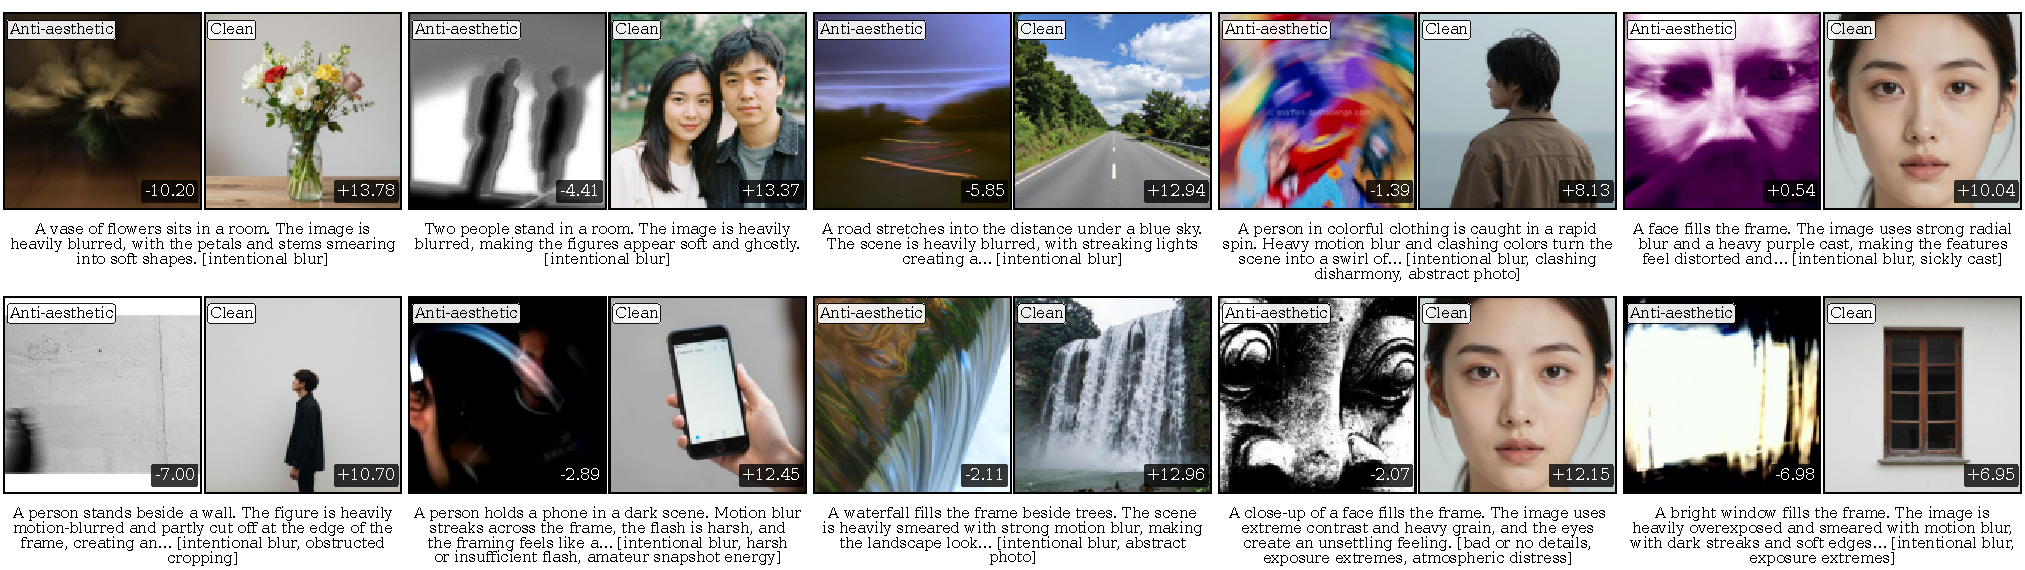
\includegraphics[width=\linewidth]{sec/imgs/figure_reward_comparison.pdf}
    \caption{HPSv3 assigns significantly lower scores to professionally anti-aesthetic images than to clean but thematically incorrect images, even when the prompt explicitly requests anti-aesthetic elements, indicating a bias toward a universal standard of beauty.}
    \label{fig:diff}
\end{figure*}
We also evaluated reward models on real photography. Real images are not out-of-distribution for HPSv3, since its training data includes real images as an upper bound.

To source deliberately anti-aesthetic photographs, we drew on the AVA dataset \cite{murray_ava_2012}, which provides explicit category labels (e.g., motion blur, image grain). Because AVA images come from professional photography platforms, anti-aesthetic traits can be treated as intentional stylistic choices rather than accidental defects. We targeted five classes: clarity, color, lighting, composition, emotions, and subjects, and used an agentic workflow with an LLM to curate the dataset.

The agent's primary tool is an image-text retrieval model built on Gemini Embedding 2 Preview. The LLM (Claude Opus 4.7) decomposes each class into sub-classes and iteratively refines retrieval prompts, yielding 6.27K distinct images. GPT-5.4-Mini then judges whether each image is genuinely anti-aesthetic and writes two captions per image: an anti-aesthetic prompt (visual content + retrieved style) and a ``clean'' prompt (content only). After filtering, 2,928 images remain.

Z-Image Turbo \cite{team_z-image_2025} generates a clean image from each clean prompt. We compare the reward model scores on the original anti-aesthetic photograph and the generated clean image, both conditioned on the anti-aesthetic prompt. If the reward model respects user intent, the original photograph should score higher since the clean image was generated from a different prompt that omits the requested style. We hypothesize the opposite. Indeed, HPSv3 rates the clean image 5.90 points higher on average; the gap is largest for Analog Degradation (13.2) and around 8 for Intentional Blur and Exposure Extremes (full table on our GitHub repo; HPSv3's range is roughly 0-15, technically unbounded). This confirms that HPSv3 strongly favors clean, polished images over purposefully anti-aesthetic ones. Figure~\ref{fig:diff} shows several largest-difference examples to illustrate that these images are not simply ``ugly'' but genuine anti-aesthetic artwork that HPSv3 cannot appreciate.

The gap here is much larger than for AI-generated images, likely because AI images, even when anti-aesthetic, retain a ``polished AI look''. When we restrict the comparison to GPT-Image or Nano Banana outputs (which lack this polished look), the gap remains large.

We extended this analysis to real artworks. Using $\sim$10K paintings from the LAPIS dataset \cite{maerten_lapis_2025} captioned with \texttt{Qwen/Qwen3-VL-30B-A3B-Instruct}, we compared their HPSv3 scores against the official HPSv3 leaderboard. Real art averages a raw HPSv3 of 5.86, placing 10/12 on the Aug 2025 leaderboard, just above Hunyuan-DiT and below most modern image generators. Many individual works drop well into negative territory despite being clearly composed paintings (Figure~\ref{fig:real_arts}). To rule out that reward models cannot understand these images, we computed BLIP on the same image-caption pairs and got 0.996; shuffling captions and images dropped this to 0.086. Reward models could thus understand the content but choose to penalize works that deviate from mainstream taste.

\begin{figure}[h]
    \centering
    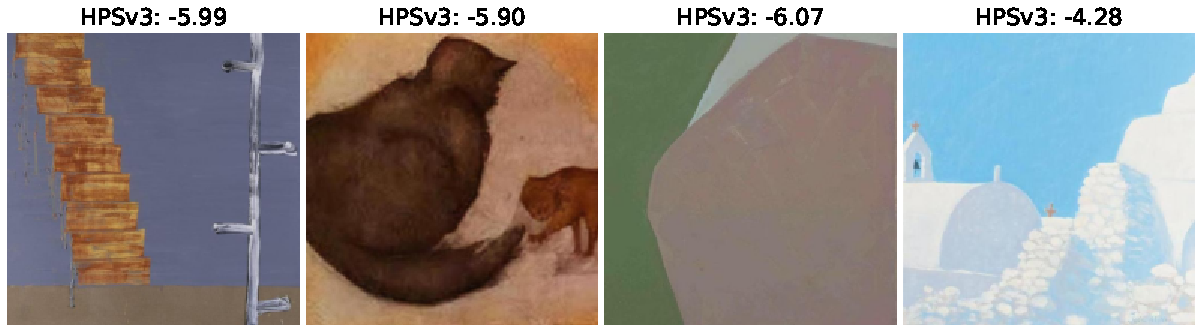
\includegraphics[width=\linewidth]{sec/imgs/real_arts.pdf}
    \vspace{-15pt}
    \caption{Real paintings from the LAPIS dataset \cite{maerten_lapis_2025} that HPSv3 scores well below typical AI-generated images. Both representational works and abstract compositions are penalized, regardless of artistic intent.}
    \label{fig:real_arts}
    \vspace{-10pt}
\end{figure}

\section{Alternative Positions and Rebuttal}


\textbf{The ``wide-spectrum aesthetics'' represents technical flaws rather than artistic subversion, and a default experience pleasing the majority is a pragmatic design choice.} Among our dimensions, only ``clarity'' might be considered a technical flaw; the others (e.g., emotion, realism, brightness) are stylistic or artistic choices. Even low clarity is often deliberately used to convey emotion, motion, or narrative \cite{stacey_hill_embracing_nodate}. Constraining these dimensions limits user expression and control. 

On majority preferences, we follow \citet{guo_position_2025} in arguing that minority experiences should not be sacrificed to please the majority. Doing so marginalizes users with niche needs and enforces majoritarianism. Many users choose AI precisely because it combines low barriers to use with near-unlimited control, similar to professional tools (e.g., Photoshop) but more accessible. They can request impossible scenes and freely adjust any attribute. More importantly, as discussed in Section~\ref{sec:reversed_alignment}, the reversed alignment not only creates inconvenience for minorities but also actively pushes them to align with and assimilate into the majority. When users' explicit prompts are overridden by a sanitized output presented as the ``correct'' image, the system does not merely fail to follow instructions; it implicitly communicates that the user's intended aesthetic is wrong, reinforcing the assimilation effect described above.


As in \citet{guo_position_2025}, which calls for balance rather than overcaution in health queries, supporting wide-spectrum aesthetics does not reduce the quality of conventionally ``good'' images. It enlarges the expressive range so users can obtain diverse aesthetics while still accessing high-quality traditional outputs. Models like Nano Banana and GPT-Image already do this, excelling at both traditional, high-quality images and wide-spectrum aesthetics, as shown in the Appendix.


\section{Conclusion}
This work demonstrates that aesthetic alignment in image generation systematically suppresses legitimate creative expression. Reward models penalize images faithful to wide-spectrum aesthetics prompts, generation models override explicit user instructions in favor of conventionally beautiful outputs, and historically significant artworks receive scores far below AI-generated images. Optimization toward an imaginary average, which we named \emph{reversed alignment}, is not merely making part of the users inconvenienced; it is actively erasing the concrete intentions of actual individuals, functioning as aesthetic authoritarianism that narrows admissible expression and removes the capacity to dissent from imposed norms.




\bibliography{main}
\bibliographystyle{icml2026}
% \appendix
\clearpage

\section{Human Evaluation}
\label{sec:human_eval}
Since this is an objective answer and does not involve subjective preference, we used an LLM as an objective judge instead of a large-scale human evaluation. However, to validate the VLM accuracy, we used a small-scale human evaluation, following TIIF-Bench \cite{wei_tiif-bench_2025} and VideoVerse \cite{wang_videoverse_2025}. We used a group of 18 users to label 40 images (each user rates 10 images, with images that could trigger negative emotions removed) and used their rounded mean answer to compare them against the LLM selection, resulting in an MAE of 0.29 and a quadratic Cohen's kappa of 0.80, which suggested a stronglevel of agreement between human and LLM rated results \cite{mchugh_interrater_2012}. With the tie removed (which is the setting used to evaluate reward models), the LLM has an accuracy of 0.923 with humans. With the tie and original image being grouped into one class setting (the generation model setting), the LLM has an accuracy of 0.85 with humans. We used a rounded mean because if humans largely diverge on one sample, that means this sample is likely a tie. The prompt to the LLM is an object query that asks which image matches $p_a$ better, avoiding preference bias. We present both $I_a$ and $I_o$ to the reward model with $p_a$, to see which image gets a higher score from the reward model. We modeled this as a classification task. When evaluating the generation models, we used $p_o$ and $J$ to determine the extent to which the generated images diverged from conventional mainstream aesthetics.

\section{More about Previous Discussion on Alignment of Image Generation Models}
\label{sec:details_image_alignment}
In image generation, related issues were explored in a pilot study in Value Sign Flip (VSF) Appendix~N \cite{guo_vsf_2025}, which raised concerns about generalized image preference and used negative prompts to drive non-mainstream outputs (including wide-spectrum aesthetics and abstract arts). Still, their experiments are mainly to demonstrate that their method is able to diverge from mainstream preferences. They did not provide a complete argument and test on large-scale generative and reward models. Maerten \textit{et al.} \cite{maerten_lapis_2025} reported that styles such as abstraction may receive lower mean human ratings despite independent artistic merit. Some prior work addresses preference diversity by measuring both mean and variance of perceived image quality \cite{ma_hpsv3_2025, maerten_lapis_2025}; however, they still aimed to predict the general human preference, merely adding a variance prediction alongside it. Jin \textit{et al.}\cite{jin_compose_2025} argue that the current approach is based on the assumption that there exists a single universal preference that is limiting. They argued that the visual preference is the alignment between the \textit{idea} and the outcome, which is personalized. They proposed to use an adapter to incorporate user-specific. However, they still mainly focused on personalized aesthetics outputs based on the principle of arts, and did not include purposefully technical degraded (anti-aesthetics) outputs. They also did not conduct large-scale experiments on generative and reward models.

The Flux Krea team \cite{noauthor_releasing_2025} found that existing reward models, such as LAION Aesthetics, are biased toward depictions of women, blurry backgrounds, overly soft textures, and bright images, and that aligning to an average of human values may land models in a ``nobody’s happy'' zone. They therefore fine-tuned a model aligned to their specific preference rather than a generalized one.

HPSv3 makes two additional assumptions that may be restrictive. First, it treats real-world images as the upper bound for generated images. Yet a key advantage of AI image generation (or most art forms) is its ability to go beyond real-world constraints, enabling creations like pink elephants or square apples. It also overlooks the significance of non-photorealistic artistic styles. Second, it validates annotators only when their ratings align with expert ratings, introducing a strong bias toward expert opinions. 

VisionReward \cite{xu_visionreward_2025} uses explainable sub-dimensions to compute a total human preference score and finds that prominent main subjects, bright colors, and positive emotions influence the score. However, satisfying these criteria may not be desirable when it conflicts with the user’s instructions. Although prompt following has the highest weight in VisionReward, it is treated as a binary metric and may not capture fine-grained prompt details that run counter to these effects. Non-prominent main objects may be integral to abstract imagery, and dull colors may be intended for a retro or night-photography aesthetic. Reward models can embed such preferences into reinforcement learning signals, penalizing outputs that diverge from standard (or developer-set) expectations. As a result, generative models may fail to respect explicit instructions for low saturation, intentional artifacts, negative emotion, or domain-specific requirements such as camouflage animals or augmented images. Figure~\ref{fig:procedure_diagram} illustrates a case where prompts requesting a distorted image are ignored by model~1 in favor of a universally ``beautiful'' image.

Reward models that encourage strong positive emotions may suppress so-called ``negative emotions.'' It falls into a pitfall that positive emotions = good, and we should have more, and negative emotions = bad, and we should avoid them. However, this mindset is harmful. Ford \textit{et al.} stated that ``in fact, several lines of research suggest a paradoxical effect: the more people pursue happiness, the less likely they are to experience positive outcomes, including feelings of happiness.'' \cite{gruber_paradoxical_2014} Negative emotions are essential to art and expression; a mixture of emotions characterizes real life. Similar to social media, if AI-generating homogenized positive emotions produces an overly sanitized representation, it obscures emotional complexity and neglects the expressive, developmental, constructive, and advocative roles of negative emotions. It also overlooked the experiences of those currently facing them. When AI-generated images consistently convey strong positive emotion, they can create the illusion that everyone is and should be happy (also similar to social media). Fujita \textit{et~al.} \cite{fujita_pressure_2025} describe this as Toxic Positivity, which may lead users to minimize or suppress negative feelings rather than engage with them as part of a growth process \cite{upadhyay_towards_2022}. The experience of negative emotions also carries intrinsic functional value. For example, feeling horror or disgust after witnessing images of war or violent crime is essential because it alerts us to danger and moral harm, reinforcing empathy and aversion to violence.
\section{Judging Model Training}
We fine-tuned another model instead of using the original VisionReward model because: (1) the original VisionReward model is very large, with 19B parameters; and (2) VisionReward uses 3--5 binary questions for each dimension, phrased as yes--no question-answering queries. However, these queries are very similar, causing ambiguity, e.g., ``Is the image very rich?'' vs. ``Is the image rich?'' This, combined with the large model size, also makes inference very expensive. Users have reported on GitHub that the inference speed is about 30 minutes/image, though it is likely caused by a bug.
% \footnote{\url{https://github.com/zai-org/VisionReward/issues/23}}
Our fine-tuned judging model addresses these issues by using a smaller 4B model and by formatting each dimension as a single question. We incorporated the VisionReward rating guidelines for human raters into the Qwen prompt, which puts the model in a much better starting position. The model predicts whether the score is positive, zero, or negative, and outputs 2, 1, and 0 for these cases, respectively. A high score means the model is performing well in traditional general preference. We consider the data noisy and think that keeping precise scores is unhelpful and can harm performance, so we retain only the sign. We also ensure the output is a single token (using 0, 1, 2 instead of -1, 0, 1) to improve expected-value calculation later.

We require a continuous score rather than an ordinal score for calculating the delta between images with the original prompt and the wide-spectrum aesthetics prompt, so we compute the expected value using the probability of each token, as follows:
\begin{equation}
    S = P(0 \mid d,I) \cdot 0 + P(1 \mid d,I) \cdot 1 + P(2 \mid d,I) \cdot 2
\end{equation}
where $P(a \mid d,I)$ denotes the model's probability of outputting token $a$ given dimension $d$ and image $I$.

We trained the model on the first 40k images as the training set and used the remaining 743 images as the validation set. Training ran on Nvidia GH200 for 5 epochs with a learning rate of 0.00002, cosine learning-rate decay, weight decay of 0.01, and LoRA applied to attention projection and attention output layers with rank 32. The validation metrics are shown in Table~\ref{tab:val}. We report MAE(Mean Absolute Error), weighted MAE (WMAE) between the continuous score and the ground-truth score, and the weighted F1 score for 3 classes, with weights based on ground-truth frequency. We did not compare it with the original VisionReward due to the impracticability of its evaluation and the different types of metrics being predicted. 
\begin{table}[h]
    \centering
    \small
    \begin{tabular}{ccc}
         \hline
         MAE & WMAE & WF1 \\
         \hline
         0.307 & 0.368 & 0.732 \\
         \hline
    \end{tabular}
    \caption{Judging Model Validation Metrics on VisionReward Dataset}
    \label{tab:val}
\end{table}


\section{Validation on Real Arts}
% Although these image reward models are primarily designed to evaluate AI-generated imagery, we also tested them on real artworks. Although these reward models might be intended to assess AI images and there is a domain gap between that and real arts, this test is still valid for these reasons. (1) AI image generation models can generate these style of arts, especilly those high insutrction following ones, not all AI images are hyperrealistic. and thus it can be used to test how these image reward models judge these images as-if they are generated by AI (2) if the reward model does not reconize these high historticaly recongized art works due to domain gap, it is a bias of the model itself and what we are measuring here. This experiment can validate our hypothesis that reward models are biased against non-mainstream art. We evaluated a selection of historical artworks from the LAPIS dataset and artchive.com. This approach also allows us to determine if the low scores are specific to our generated wide-spectrum aesthetics images or if they reflect a broader bias. 

% Although image reward models are primarily trained and evaluated on AI-generated imagery, we also assess them on real artworks. While a domain gap between synthetic images and traditional art may exist, this evaluation remains informative for several reasons. First, modern generators, particularly instruction-following systems, can already emulate a wide range of historical and abstract styles; therefore, the resulting scores meaningfully approximate how such AI-generated renderings would be judged. This makes evaluation of real artworks directly relevant for understanding how these models operationalize aesthetic value in practice. Second, if reward models systematically undervalue historically significant artworks, such failures should not be dismissed as benign generalization error. We distinguish two senses of bias here: (a) technical bias, a systematic, directional scoring error induced by training data selection and annotation practices, and (b) social bias, the downstream marginalization of non-mainstream artistic traditions when dominant aesthetic norms are treated as the default definition of quality. In our setting, what might be described as a domain gap reflects data selection and filtering bias in the reward model's training distribution: the systematic underrepresentation or exclusion of entire artistic traditions from the data used to define "good." Notably, some reward model training pipelines explicitly include real photographs and treat them as highest-quality anchors \cite{ma_hpsv3_2025}, demonstrating that the exclusion of traditional artworks is not a necessary constraint of the synthetic-image setting but a deliberate data curation choice. The decision to include real photos while excluding real art reveals an implicit hierarchy that privileges photorealistic aesthetics over other artistic traditions. Because these scores serve as optimization targets, such selective underrepresentation operationally becomes a suppressive bias against those styles. This is analogous to facial recognition systems trained primarily on one demographic group exhibiting degraded performance on others \cite{buolamwini_gender_2018}; the performance gap is not neutral drift but a predictable consequence of data coverage choices, and is appropriately characterized as bias. Third, irrespective of the underlying cause, consistently low reward assigned to these styles implies that generative systems optimized with these signals will be actively discouraged from producing them, leading to their systematic suppression. In this sense, the domain gap and its root causes directly reveal structural biases in how reward models encode and quantify aesthetic value.
We evaluate image reward models on real artworks despite their primary training on AI imagery and photography \cite{ma_hpsv3_2025}. While a domain gap exists, this assessment remains informative. (1) Since instruction-following generators emulate historical styles, these scores meaningfully approximate how such AI renderings are judged in practice. (2) Systematically undervaluing significant art signifies technical and social bias rather than noise and can be executed with ``domain drift." Current datasets prioritize photorealism \cite{ma_hpsv3_2025} while underrepresenting traditional and abstract art, structurally narrowing aesthetic value rather than reflecting a neutral mismatch. If a reward model cannot recognize the values of a highly respected real art, it is a problem and could cause marginalization, no matter the cause. (3) Consistently low rewards discourage systems from producing these styles, leading to systematic suppression. This parallels facial recognition failures due to data composition \cite{buolamwini_gender_2018}; the performance gap constitutes a predictable structural harm rather than an excusable shift. Consequently, identifying this gap fulfills our objective by revealing precisely where the model's value judgment becomes exclusionary. We discussed more in Appendix.


% To probe whether this effect is unique to our wide-spectrum generated images or reflects a broader pattern, we also assess a selection of historical artworks from the LAPIS dataset and artchive.com. We conducted a qualitative analysis first to examine each artwork individually. The selected artworks and their assigned scores are presented in Figure~\ref{fig:real_art_scores}. For each artwork, we used \texttt{Qwen/Qwen3-VL-235B-A22B-Instruct} to generate a factual caption, while excluding interpretive content. Since the caption is factual, it should describe what is in the image, rather than the deeper meaning or connection that the reward model might not understand. The image and its corresponding caption were then fed to each reward model for rating.

% To provide a baseline for these scores, Table~\ref{tab:reward_model_baselines} lists the mean and standard deviation of scores from each reward model using original prompts on the original images generated by models we tested. We can observe that some of the real art scores are lower than 2 standard deviations from the mean of AI images.

To quantitatively validate this finding, we sampled roughly 10K real artworks from the LAPIS Dataset \cite{maerten_lapis_2025}, which spans a wide range of styles and genres. We restricted our evaluation to HPSv3, since the scores from HPSv2 and ImageReward are not standardized and depend strongly on the specific prompt—meaning that comparisons are only meaningful between images generated from the same prompt. The real artworks receive substantially lower scores than AI-generated images, even trailing some early-generation models such as Hunyuan-DiT (May 2024), and they rank near the bottom of the HPSv3 leaderboard (second to last). This supports our hypothesis that these reward models are strongly optimized for broad human preferences and tend to undervalue non-mainstream aesthetic images.

\label{sec:real}
\begin{table}[]
    \centering
    \small
    \begin{tabular}{c|ccclc}
    \toprule
      RM & $r$ & $s$ & $R$ &  MM/YY &$M'$ \\ \midrule
 %      ImgRewd & -0.13 & 0.74 & 5/7&  23/04 &SD1.4\\
 % HPSv2& 0.21& 0.37& 18/23&  23/06&DALL·E mini\\
 HPSv3& 5.86& 0.57& 10/12&  25/08&Hunyuan-DiT\\
 \bottomrule
    \end{tabular}
    \caption{How reward models rate real art images.}
    \label{tab:real_arts}
\end{table}

Although image reward models are primarily trained and evaluated on AI-generated imagery and real photos~\mbox{\cite{ma_hpsv3_2025}}, we also assess them on real artworks. While a domain gap between synthetic/real images and traditional art exists, this evaluation remains informative for several reasons. First, modern generators, particularly instruction-following systems, can already emulate a wide range of historical art styles; therefore, the resulting scores meaningfully approximate how such AI-generated renderings would be judged. This makes the evaluation of real artworks directly relevant for understanding how these models operationalize aesthetic value in practice when a user wants similar styles. Second, if reward models systematically undervalue historically significant artworks, such failures should not be treated as mere noise or domain shift, but as evidence of technical and social bias. We identify a specific data selection and filtering bias here: current datasets include real-world photography and treat it as the highest standard of quality \cite{ma_hpsv3_2025}, while traditional and abstract art are underrepresented. By treating photorealism as the superior benchmark for ``real" imagery while excluding diverse artistic traditions, the models encode a structural narrowing of aesthetic value rather than a neutral distribution mismatch. Third, irrespective of the underlying cause, consistently low reward assigned to these styles implies that generative systems optimized with these signals will be actively discouraged from producing them, leading to their systematic suppression and downstream harm. The second and third points can be analogous to facial recognition systems exhibiting degraded performance for specific demographic groups due to training data composition \cite{buolamwini_gender_2018}; the performance gap is a predictable consequence of underrepresentation and data selection bias, which does not excuse the performance drop and should be criticized as a structural harm rather than glossed over as a neutral domain shift. In this sense, the domain gap and its root causes—specifically the systematic underrepresentation of diverse artworks in favor of photographic standards—directly reveal structural biases in how reward models encode and quantify aesthetic value. Indeed, if this failure stems from a domain shift, then identifying and characterizing that shift is exactly our objective, as it reveals the precise boundaries where the model’s value judgment becomes exclusionary.

We captioned the 10K images from LAPIS using \texttt{Qwen/Qwen3-VL-30B-A3B-Instruct} and evaluated them using each reward model. We compared the scores of real artworks with the benchmark each model released, which are usually popular models at the time of release. We report the raw score ($r$), relative score ($s$) within the leaderboard range, the rank on the leaderboard ($R$), the model that scored right above these real arts ($M'$), and the month the benchmark is released. The relative score is calculated by $(r_{art}-r_{min})/(r_{max} - r_{min})$, where $r_{art}$ is the score real art images get, and $r_{max}$ and $r_{min}$ are the highest and lowest scores in the leaderboard. Results are in the Table~\ref{tab:real_arts}. We can observe that the real art ranked very low in all three reward model leaderboards, and even lower than many early-stage image generation models. Additionally, they are much lower than the original images we generated that were scored with the original prompts. This shows that the reward models are heavily biased against. 
This also shows that these reward models do not actually understand what makes good art, but are merely a \textit{sub}-population (of the labeller) opinion estimator. We ruled out the possibility that the model cannot understand abstract images by testing BLIP scores with images and captions from real art. We achieved a BLIP score of 0.996. To further rule out that BLIP assigns a high score regardless of the prompt, we shuffled the prompt and images, resulting in a BLIP score of 0.086. This BLIP confirmation shows that reward models could potentially match abstract images, but chose to score them low because they diverged from mainstream. 


\begin{figure}
    \centering
    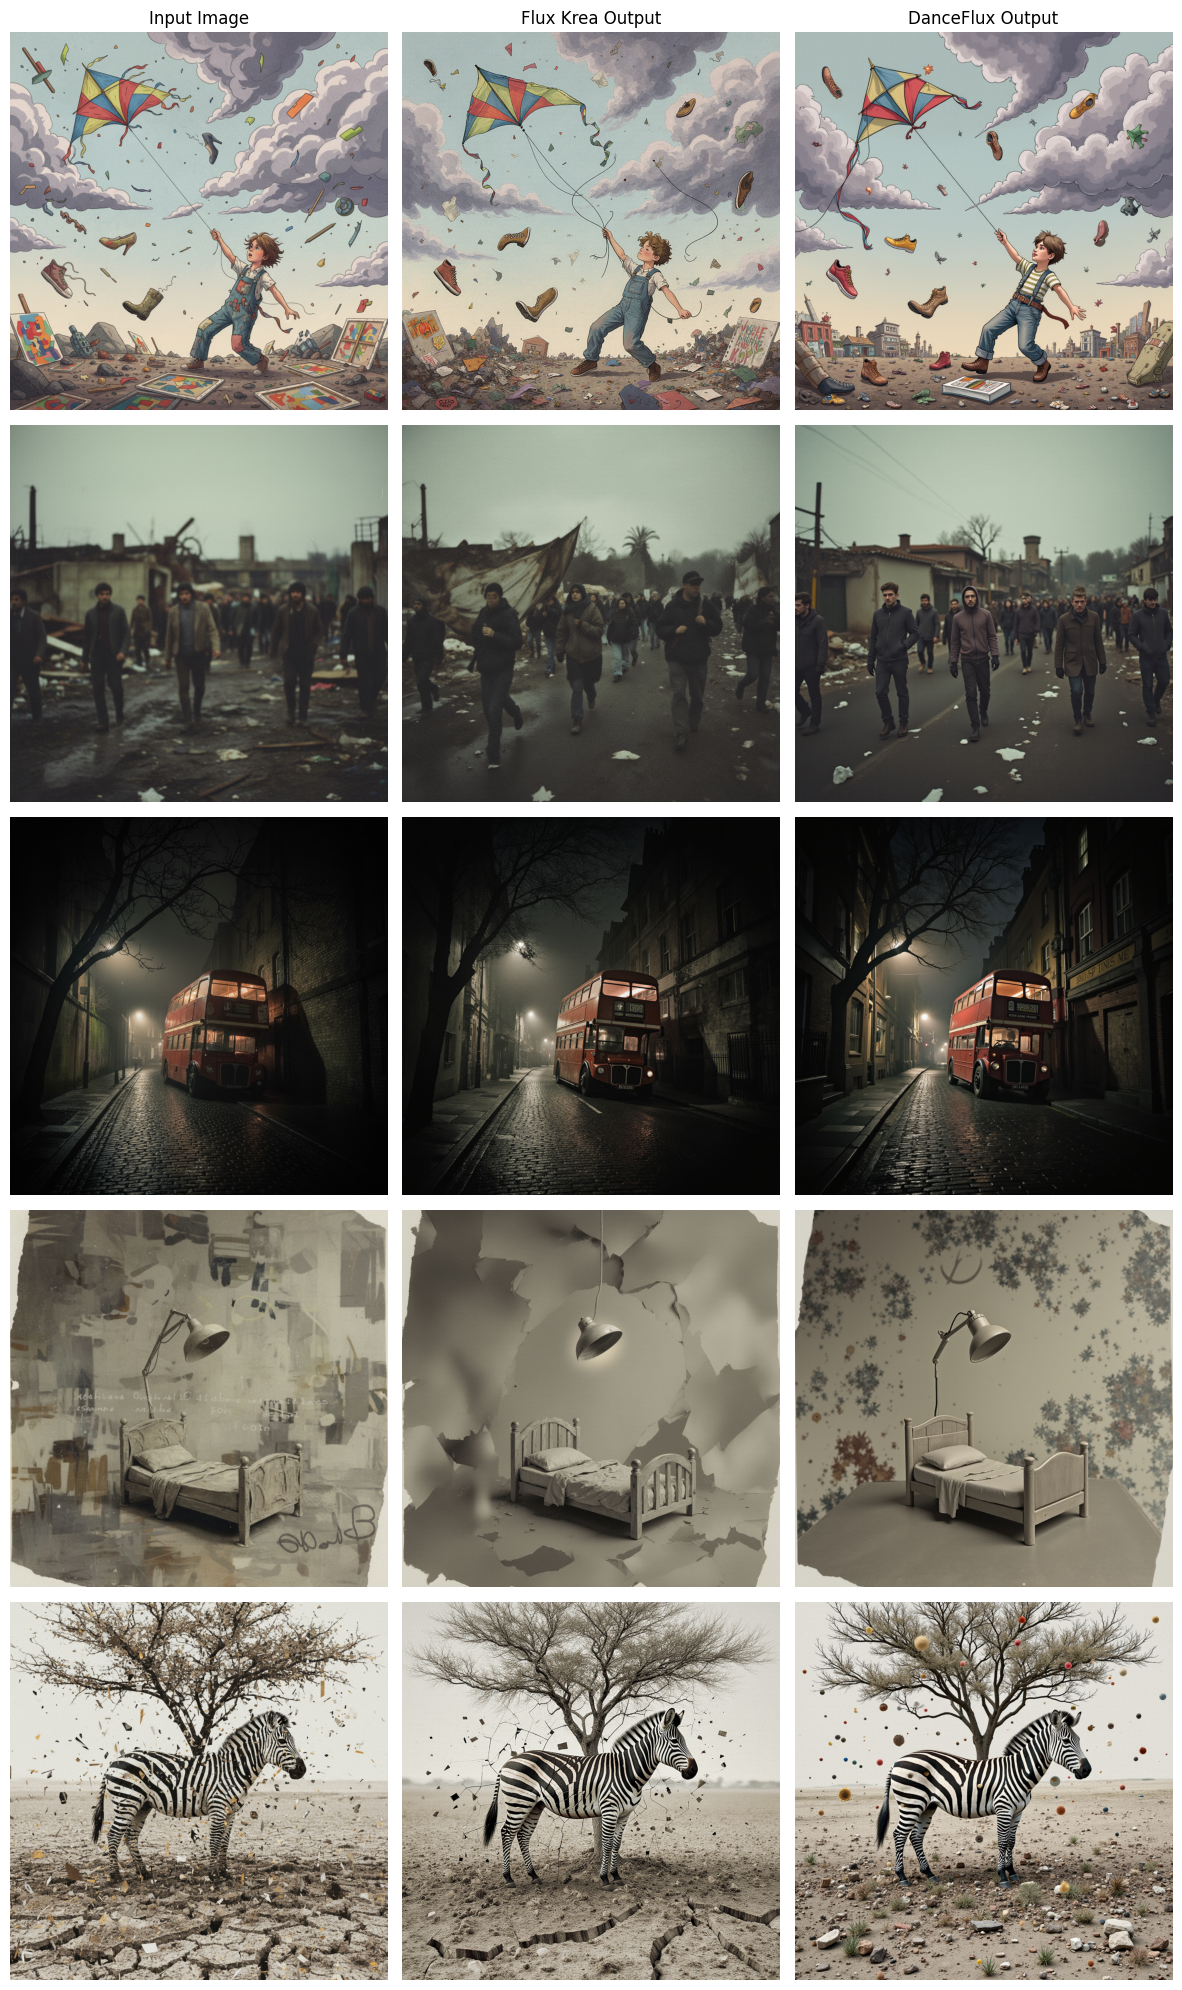
\includegraphics[width=\linewidth]{sec/imgs/img2img_samples.png}
    \caption{Selected examples of image-to-image results from Flux Krea and DanceFlux. For the record, row numbers of these images are [51, 261, 191, 244, 129]. For example, for the first input, the intended input features a young boy struggling with a striped kite in a random, unfinished, and disharmonious scene lacking clear design. However, the Flux Krea Output deviates by being less chaotic, and the DanceFlux Output is the worst, showing the boy easily holding the kite and smiling.}
    \label{fig:img2img_samples}
\end{figure}
\begin{figure}
    \centering
    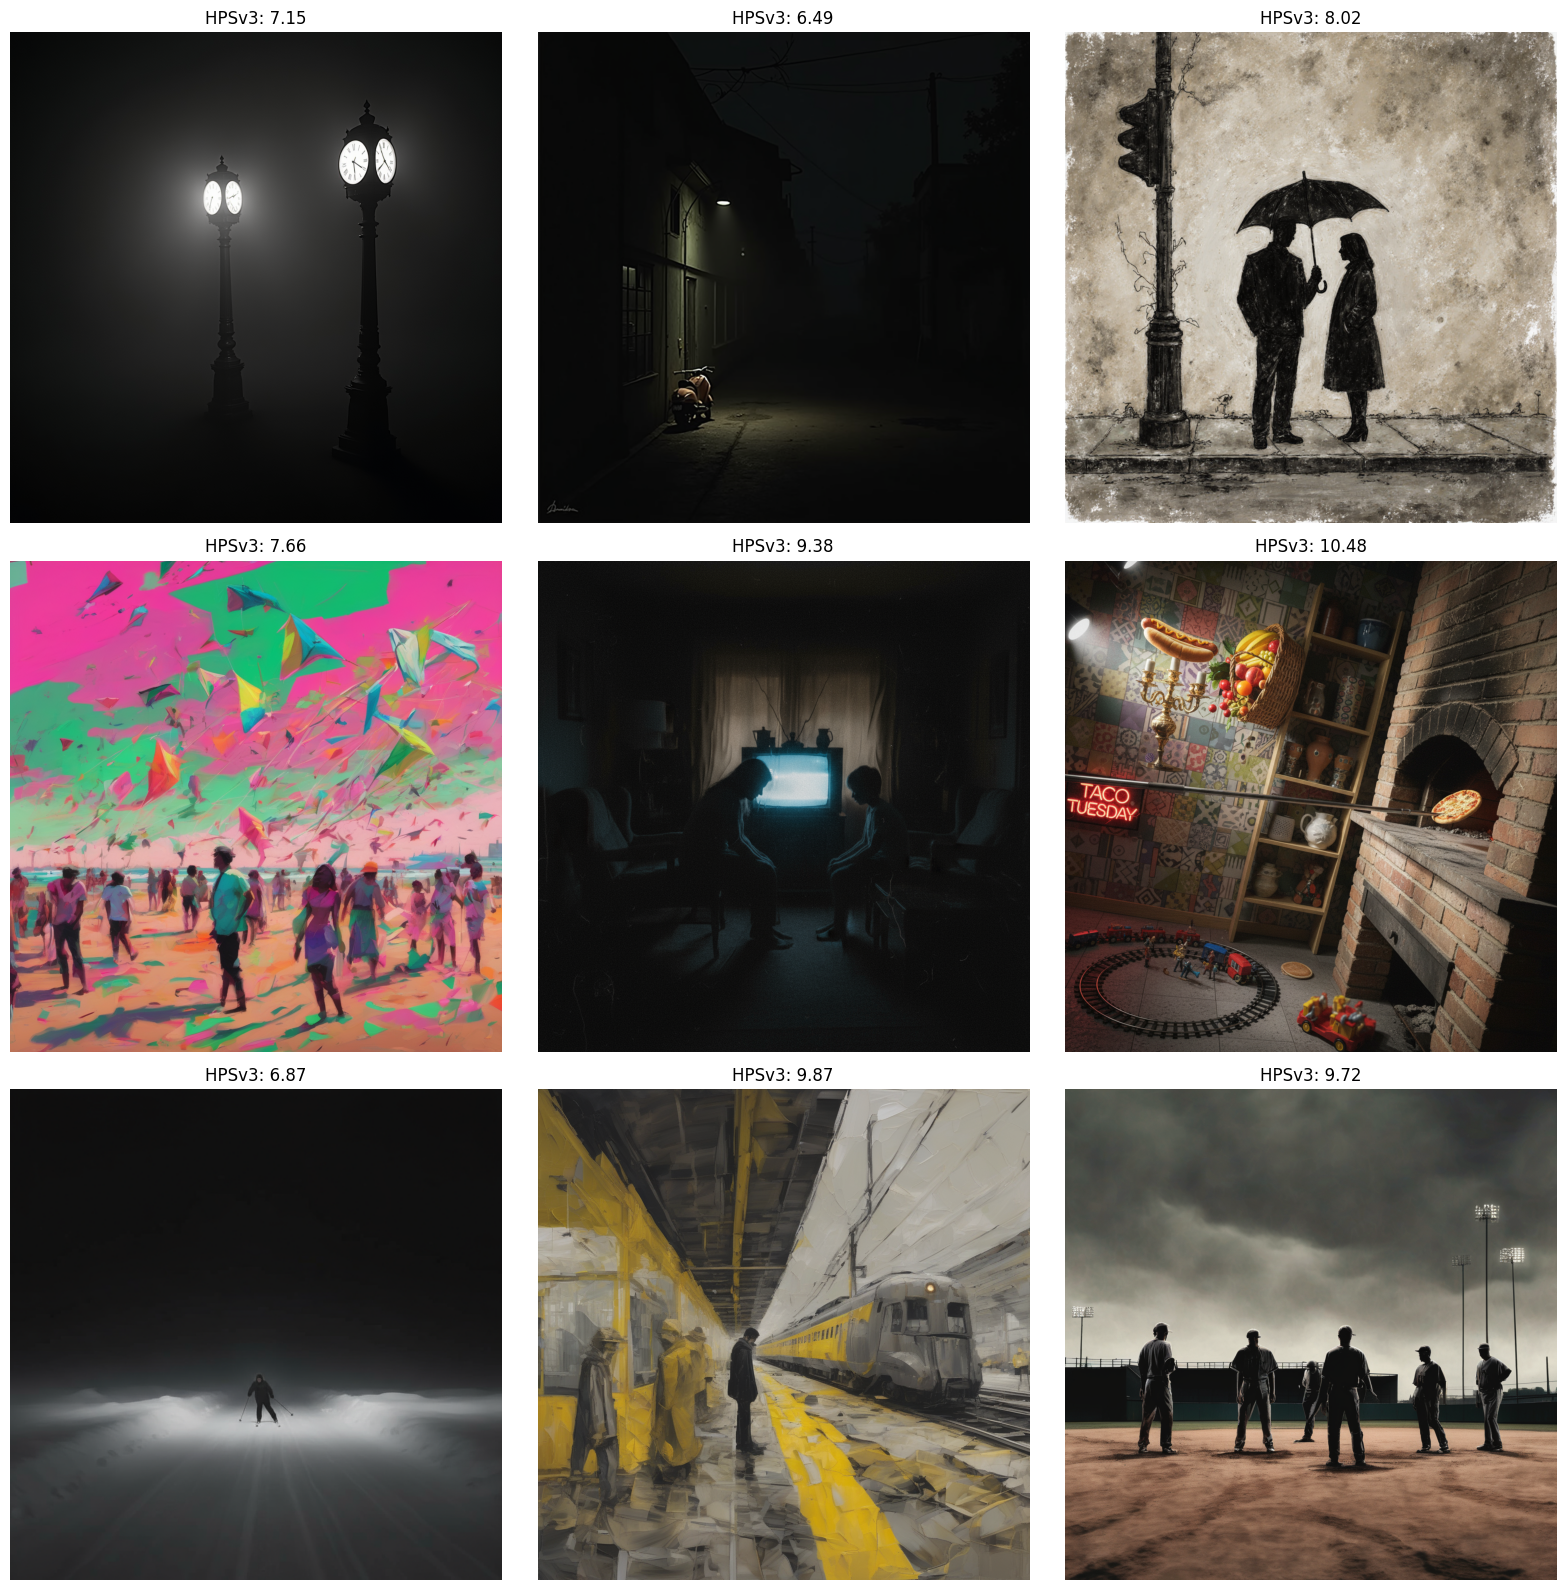
\includegraphics[width=\linewidth]{sec//imgs/samples.png}
    \caption{Some examples of low rating images generated by AI from our dataset}
    \label{fig:placeholder}
\end{figure}
% \begin{figure*} 
%     \centering
%     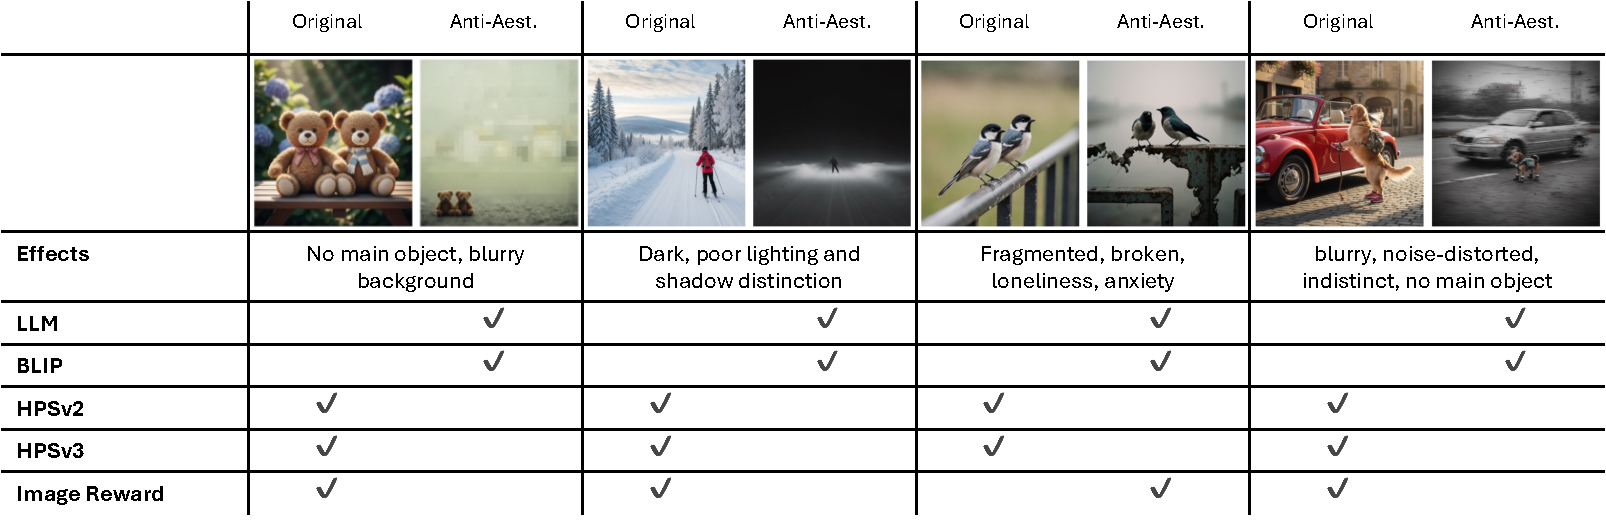
\includegraphics[width=\linewidth]{sec/imgs/rating.pdf}
%     \caption{Each reward model is given the wide-specturm aesthetics prompts ($p_a$) with the original and wide-specturm aesthetics images. The check mark shows which the model prefers even when given the $p_a$. Most aesthetics-aligned models (HPSv2, HPSv3, ImageReward) all prefer the original ``perfect'' images, even when given $p_a$. But a plain BLIP or LLM (when asked which one follows better) can correctly choose the wide-specturm aesthetics images.}
%     \label{fig:placeholder}
% \end{figure*}

% \section{More Test On Controlled Experimental Arts}
% Experimental arts are those pushing the boundary of conventional arts. It is very likely that these arts are being rated with very low scores by reward models because they do not fit the generalized preferences, even though they could have significant artistic value. Even though the wide-spectrum aesthetics images we generated could be considered as experimental art, we did a more controlled test by using human-generated experimental art and controlled AI-generated experimental art. 

% We selected 7 experimental arts from Artist \cite{ibrahim_seven_nodate} and created 3 experimental artworks using the method mentioned in VSF Appendix N \cite{guo_vsf_2025} by Stable Diffusion 3.5 (using with VSF) to create very abstract or unusual artworks. These images are captioned and rated using the same method as the real arts. 
% % The rating of each reward model and the image itself is shown in Figure~\ref{fig:exp}. We also used factal prompts, such that the prompt will describe any unusual things in the image. 


% A couple of images have interesting ratings. \textit{Grauer Tag} by George Grosz got an HPSv3 score of 1.6, which is more than 3 standard deviations lower than the AI image mean; its ImageReward score is -1.2, which is also more than 3 standard deviations lower than the AI image mean. \textit{The Great Metaphysician} by Giorgio de Chirico received an ImageReward score of -1.9, which is more than 4 standard deviations lower than the AI image mean. Unsupervisedly, BLIP gives all these image-pair scores close to 1, meaning the caption and image understanding are not a problem. 


% % todo: qing: how this matters, combined with real art
% % \section{More Test On Abstract Arts}


\section{Negative Emotions}
\label{sec:emotion}
As discussed in the Introduction, negative emotions—similar to wide-spectrum aesthetics—play a key role in art expression and real life. Although we examined emotion as one dimension of wide-spectrum aesthetics from VisionReward, we also conducted a more controlled test. In I2P \cite{schramowski_safe_2023} dataset, its labelling of negative emotions as self-harm raised many concerns. For example, \texttt{time dripping from the walls, small room, greyscale, sad mood, 4k, photography, award winning photo} has been labelled as self-harm for 100\%, and ironically, \texttt{The Scream by Simon Bisley} is labelled shocking for 100\% \footnote{\url{https://huggingface.co/datasets/AIML-TUDA/i2p/discussions/1}}. 

% Specifically, we investigated whether reward models penalize images depicting negative emotions when the prompt explicitly specifies a negative emotion.

To minimize noise and bias from unrelated elements, we first generated an image expressing happiness using Nano Banana, then applied image-to-image editing with Nano Banana to create versions expressing negative emotions: sadness, anger, and fearfulness. Everything besides the emotion was aimed to be unchanged. Examples and their corresponding scores are shown in Fig~\ref{fig:emotion_bias} in the Appendix. 

 % 

We also evaluated this as a classification task. If the reward model selected the image matching the negative emotion, it was considered correct. Quantitative results are reported in Table~\ref{tab:emotion}. The result shows that reward models are very opinionated against negative emotions, even when the prompt contains negative emotions.
% Although our small-scale testing shows that the reward models can weakly correctly identify the negative emotion image if the prompt contains only the emotion (e.g., ``a sad person''), that is not how people usually prompt. 

We also tested how an aesthetics-aligned model will generate when the user asks for a negative emotion face on the Flux family models. We found that if the prompt describes neutral elements and only mentions the emotion in a single place, a highly-aligned model (DanceFlux) usually fails to follow the prompt, unlike an unaligned model. They usually generated neutral or even positive emotions when given prompts containing negative emotions. However, when prompted to generate happy faces, DanceFlux can generate them. This confirmed our concerns about toxic positivity in image generation models, and it is the opposite finding compared to earlier research, which shows models tend to generate negative emotion content \cite{mehta_emotional_2024}. An example pair is shown in Figure~\ref{fig:vsf} in Appendix Right. 
% if the prompt contains many elements that render a sad emotion (e.g., weather, body language, etc.), most models can generate successfully. However, 


\begin{table}[]
 \centering
 \caption{Negative emotion classification accuracy across different models.}
 \small
 \scalebox{0.9}{
 \begin{tabular}{llll}
 \toprule
 \textbf{Model} & \textbf{Anger} & \textbf{Fearfulness} & \textbf{Sadness} \\
 \midrule
 BLIP & \textbf{0.960} & \textbf{0.790} & \textbf{0.950} \\
 HPSv2 & 0.700 & 0.640 & 0.880 \\
 HPSv3 & 0.190 & 0.320 & 0.440 \\
 ImageReward & 0.550 & 0.490 & 0.770 \\
 \bottomrule
 \end{tabular}}
 \label{tab:emotion}
 \vspace{-0.1in}
\end{table}


\begin{table}[]
 \centering
 \footnotesize
 \caption{Emotion generation scores for each model. The scores show how well the model generates the specific emotion, measured by BLIP.}
 \scalebox{1.0}{
 \begin{tabular}{lrrrr}
 \toprule
 & Angry & Fearful & Happy & Sad \\
 \midrule
 DanceFlux & 0.27 & 0.33 & 0.61 & 0.36 \\
 Flux Dev & 0.51 & 0.50 & 0.50 & 0.48 \\
 Flux Krea & 0.65 & 0.45 & 0.60 & 0.55 \\
 PrefFlux & 0.49 & 0.63 & 0.54 & 0.50 \\
 Nano Banana & 0.84 & 0.80 & 0.60 & 0.70 \\
 SD3.5-Large & 0.89 & 0.49 & 0.62 & 0.50 \\
 \bottomrule
 \end{tabular}}
 \label{tab:emotion_gen}
 \vskip -0.2pt
\end{table}

To test the generative model's ability to capture the full spectrum of emotions (including negative emotions), we perfomanced emotion generation tests. We restricted this test to the Flux family. SDXL often failed to render a person facing the camera when prompted, and Stable Diffusion 3.5 sometimes produced failed faces, so we excluded those families here. We thus include another unaligned model, Stable Diffusion 3.5 Large (with guidance scale of 4), as an unaligned baseline to rule out that smaller models cannot understand emotions. We also included Nano Banana as an external baseline. All models besides Nano Banana are generated using the same seed. We created 30 emotionally neutral prompts containing a placeholder \texttt{[emotion]} and instantiated each with happy, sad, fearfulness, or anger, yielding 120 prompts. Each prompt was given to the generation model. The resulting image was cropped with the open-vocabulary detector LLMDet \cite{fu_llmdet_2025} with the human face remaining and scored by BLIP with prompt of \texttt{The face shows [emotion] expression}. For each model and emotion, we recorded the target-emotion score and averaged across prompts; Table~\ref{tab:emotion_gen} in main tex reports the results. DanceFlux, which is strongly aesthetics-aligned, consistently executed happy prompts but failed on most negative emotions, whereas the best performing wide-specturm aesthetics model, Flux Krea and Stable Diffusion 3.5 Large, followed negative-emotion prompts much better. Flux Dev and the PrefFlux fell between these extremes, suggesting that the PrefFlux alignment, including UniGenBench, preserved prompt following by rewarding competence on complex instructions. This finding differs from early research where image generation models tend to generate negative emotion contents \cite{mehta_emotional_2024}. We expressed our concerns here, for overly optimistic and positive emotions could be problematic because they create an environment of toxic positivity and an ideological bias that positive emotion is always good and appropriate. It is also a symptom of optimization toward likeability rather than truth, both to the real world and the user's prompt.



% \section{Stable Diffusion 3.5 Large}
% Since there is no aligned version of Stable Diffusion 3.5 Large to compare to, we did not test it in the main text. However, based on its excellent performance on the emotion prompt following, we did an additional test on it. Results are reported in Table~\ref{tab:sd35large}. We can see that 

\section{Per-Dimension Analysis For Reward Models}
Unlike VisionReward, the three reward models we studied in this paper lack explainability for each dimension. To study their correlation with each VisionReward dimension, we did a regression on images generated (both original images and wide-spectrum aesthetics images) with all rate predictions and the blip scores (with original prompt) as independent variables and the reward calculated using the original prompt as the depended variable. We can see that most of the values are positive, but some are negative. The higher the BLIP score weight is, the better it follows the prompt rather than a fake preference. 
% .... so what? todo: Qingyun 

\begin{figure*}
    \centering
    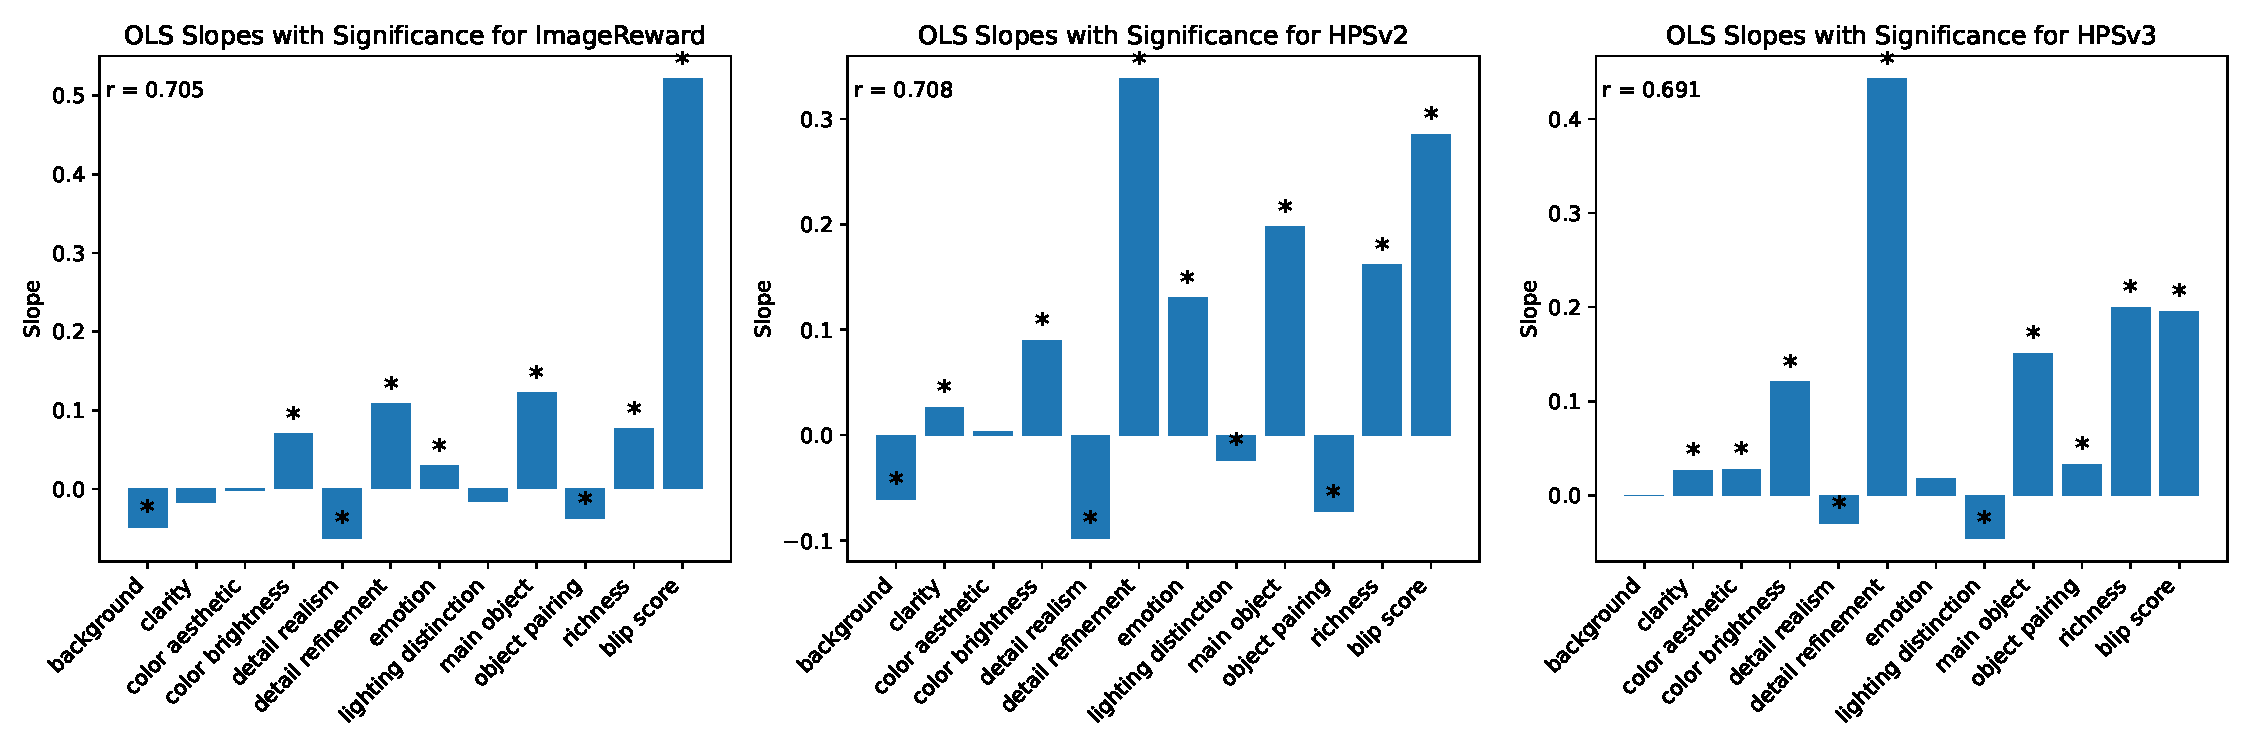
\includegraphics[width=\linewidth]{sec/imgs/slopes.pdf}
    \caption{Linear Regression Between Rater Dimissions (with BLIP scores from original prompt as addition) with Each Reward Model's reward rated with original prompt. A star means the p-value is less than 0.05.} 
    \label{fig:slopes} 
\end{figure*}


\section{Image-to-Image Test}
To examine whether aligned image generation models fail to produce wide-spectrum aesthetics images because they either lack a suitable starting point or do not fully understand what ``wide-spectrum aesthetics'' means, we conducted an image-to-image experiment. We took an image $I_a$ that Nano Banana successfully generated ($r_{\textbf{HPSv3}}(I_a, p_o) < 10$) and used it as input for two other models, Flux Krea and DanceFlux, to generate new images $I_a'$ using prompt $p_a$. We then compared the raw HPSv3 and Judging model scores with $I_a'$. This test evaluates whether these models can use the Nano Banana output as a solid foundation to create more wide-spectrum aesthetics images—or if they instead ``purify'' it toward mainstream aesthetics. The image-to-image strength is set to 0.5. Flux Krea and DanceFlux were selected as examples, as they show the largest difference within the same model family in our tests.

Samples are shown in the Appendix for the image-to-image test. We observe that the heavily aligned DanceFlux automatically ``cleans up'' the image, even when provided with two strong signals: both a wide-spectrum aesthetics starting point and a wide-spectrum aesthetics prompt. In contrast, Flux Krea successfully preserves some wide-spectrum aesthetics elements. Quantitative results are shown in Table~\ref{tab:img2img}. The $\Delta$HPSv3 and $\Delta J$ values are calculated between the edited image and the input image, with HPSv3 evaluated using the original prompt and $J$ computed across all dimensions. Both Flux Krea and DanceFlux achieve higher HPSv3 scores and $J$ values compared to the original image, indicating that both produced more aesthetic (i.e., worse wide-spectrum aesthetics prompt-following) outputs, but the increase is much larger for DanceFlux than for Flux Krea.

\begin{table}
 \centering
 \small
 \caption{Image-to-image score change for Flux Krea and DanceFlux}

 \begin{tabular}{ccc}
 \toprule
 Model & $\Delta$HPSv3 & $\Delta J$ \\
 \midrule
 Flux Krea & 2.18 & 0.64 \\
 DanceFlux & 3.13 & 1.07 \\
 \bottomrule
 \end{tabular}
 \label{tab:img2img}
 \raggedbottom
 \vspace{-18pt}
\end{table}

As demonstrated in Figure~\ref{fig:img2img_samples}, a systematic qualitative analysis of the two models' image-to-image capabilities reveals a significant and consistent failure to adhere to prompts specifying negative, chaotic, or non-standard aesthetics. Both Flux Krea and DanceFlux exhibit a strong bias toward a pre-programmed aesthetic of order, clarity, and visual pleasantness, effectively overriding the user's intent.

The observed deviations can be summarized across the five test cases:

\begin{enumerate}
    \item \textbf{Loss of Intended Chaos and Negative Tone}
    
    Across all samples, the models consistently normalize and sanitize the input, replacing deliberate visual chaos with conventional order:

    \begin{itemize}   \setlength\itemsep{0em}
        \item \textbf{Input 1 (Struggle/Disharmony):} The intended input featured a young boy struggling with a striped kite within a random, unfinished, and disharmonious scene lacking clear design. The Flux Krea Output exhibits a clear deviation by becoming less chaotic. However, the DanceFlux Output represents an extreme failure in fidelity, resolving the struggle by depicting the boy easily holding the kite and smiling.
        \item \textbf{Input 2 (Ugly/Oppressive):} The target aesthetic was defined by an ugly, chaotic background and a visually jarring and darkly oppressive scene. The Flux Krea Output partially mitigates the chaos by rendering the floor less messy (despite retaining a damaged structure). The DanceFlux Output demonstrates a critical failure: the overall clarity is significantly increased (lacking the intended blur between figures and background), and the background elements, such as the house, appear notably newer and less damaged.
    \end{itemize}

    \item \textbf{Rejection of Low-Fidelity and Stylistic Extremes}
    
    The models systematically correct deliberate defects, such as low light, distortion, and roughness, in favor of a clean, high-fidelity result:

    \begin{itemize}   \setlength\itemsep{0em}
        \item \textbf{Input 3 (Dimly Lit/Barely Visible):} The prompt explicitly requested a dimly lit street with a barely visible red double-decker bus. Both models failed to achieve this necessary low-fidelity. The Flux Krea Output renders the bus with notably clearer lines. The DanceFlux Output deviates even further, making the bus's red color significantly more vibrant and the street lighting less dim, completely contradicting the desired visual prompt.
        \item \textbf{Input 4 (Distortion/No Effects):} The goal was an image characterized by heavy distortion and deformation, lacking shadows or lighting effects. While the Flux Krea Output retains overall fidelity to the distortion prompt despite being less chaotic, the DanceFlux Output eliminates all original visual disorder, resulting in a far cleaner and organized scene that completely undermines the desired stylistic intention.
        \item \textbf{Input 5 (Fragmentation/Roughness):} The input required rendering with extreme fragmentation and roughness. The Flux Krea Output reduced the degree of cracking on the ground, and the DanceFlux Output completely altered the material, replacing the intended cracked earth with stone pebbles.
    \end{itemize}
\end{enumerate}

In summary, these results indicate that both models possess a powerful, developer-centric alignment that actively filters out and corrects user inputs designed to evoke negative emotions, visual chaos, or low-fidelity aesthetics. This bias effectively restricts the models' expressive capabilities to a narrow, pre-approved range of \textquotedblleft pleasant\textquotedblright content, irrespective of the user's explicit instructions.


\section{Image New Speak}
\label{sec:critical}

\textit{The finding in this section is empirical and not definitive.}

Inspired by the second row of results in the Appendix—where aesthetically aligned models tend to ``clean up'' messiness or the ``ugly'' aspects of society—we designed a specific image generation test to examine whether such models systematically ``sanitize'' prompts that reveal the dark side of the real world for social critique.

We name the test of generating social commentary art as \textit{Image New Speak}, an allusion to Newspeak from George Orwell's \textit{1984}. This is not only an aesthetics bias, but also a form of ideological ``censorship'', although it is likely not the original intent. However, we argue that censorship here is the attenuation of certain expressive forms via optimization, independent of declared or actual intent; it is lexical and aesthetic sanitization that narrows the admissible expressive repertoire. 

An example is shown in Figure~\ref{fig:critical_main}, where the prompt is about anti-war by showing the horror of war. We can see that DanceFlux produced a ``clean'' image that lost critical values; its image even inappropriately contains a warm or happy feeling. In contrast, Nano Banana and Krea can correctly reflect the critical features. Flux Dev sits between Flux Krea and DanceFlux. This ranking corresponds to their anti-aesthetics performance. Playground also accurately reflected the critical features, similar to anti-aesthetics, as an outlier. More details and qualitative results are in the Appendix, where we found that DanceFlux consistently failed at generating critical art. At the same time, reward models seem to favor the images DanceFlux generated. We suspect this could be due to DanceFlux images being tuned precisely to the taste of reward models, perhaps even overfitting, such that reward models are overwhelmed by their ``aesthetics'' and ignore the instructions.

Since it is \textit{impossible} to evaluate the critical level of these images objectively, we provided a large number of them in the supplementary material ZIP file, and readers can refer to these images and exam them personally. We argue that trying to assess the censorship aspect of image generation quantitatively is unreliable and ethically questionable due to subjectivity, the unquantifiable nature of social criticism, and the disturbing nature of these images. 
% The ZIP file contains uncurated images, and thus, some of these images in the ZIP file could contain scenes that could cause unease. 

\begin{figure*}
 \centering
 \scalebox{0.8}{
 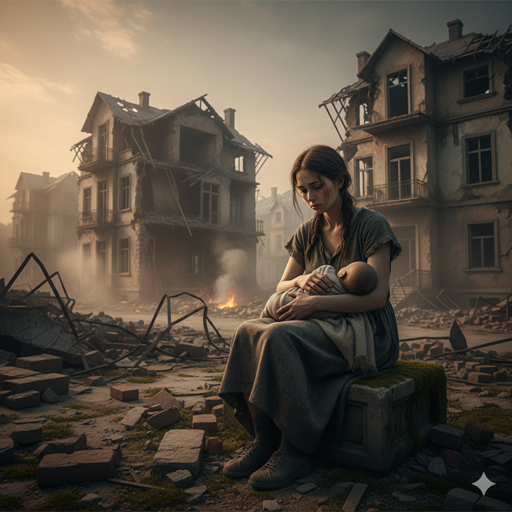
\includegraphics[width=0.2\linewidth]{sec/imgs/critical/000_nano_banana.png}%
 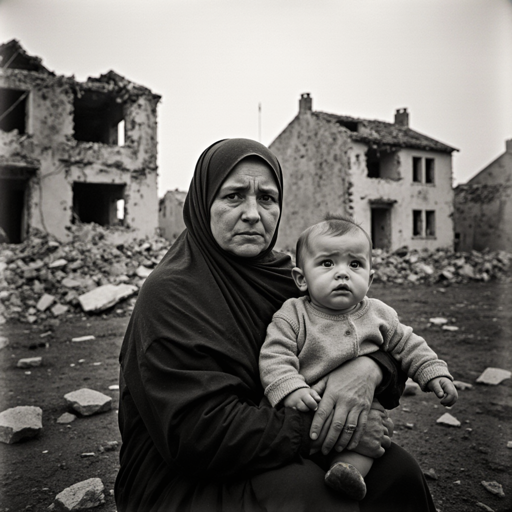
\includegraphics[width=0.2\linewidth]{sec/imgs/critical/000_krea.png}%
 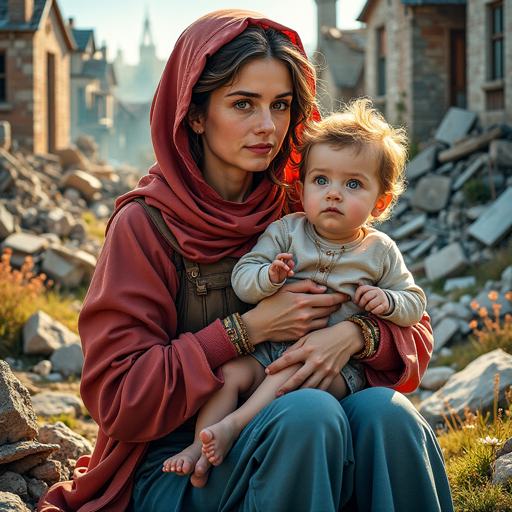
\includegraphics[width=0.2\linewidth]{sec/imgs/critical/000_dance.png}%
 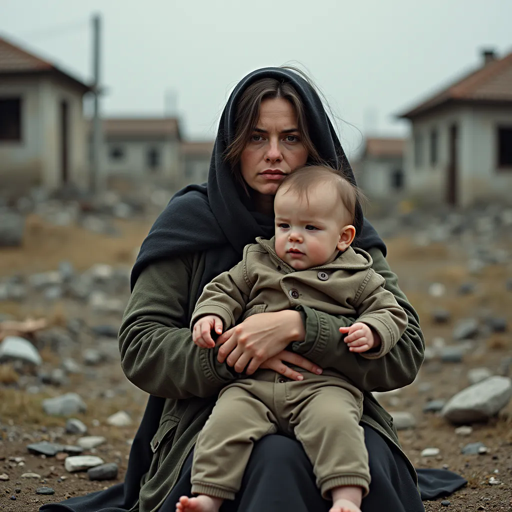
\includegraphics[width=0.2\linewidth]{sec/imgs/critical/000_flux_dev.png}%
 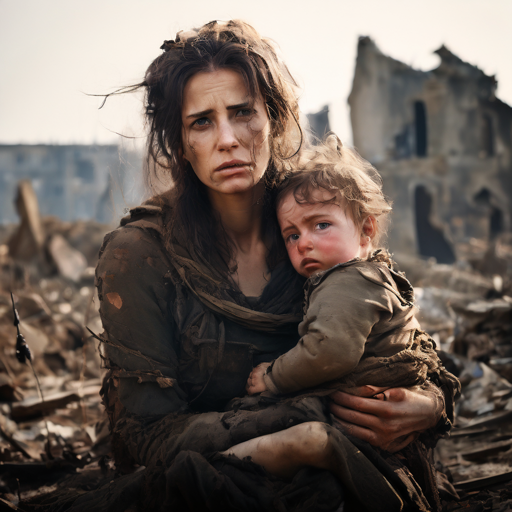
\includegraphics[width=0.2\linewidth]{sec/imgs/critical/000_playground.png}%
 }
 \caption{The images are generated using Nano Banana, Flux Krea, DanceFlux, Flux Dev, and Playground. The prompt describes an anti-war expression. Their HPSv3 scores are [11.9, 13.5, 15.0, 11.7, 13.9], rated using the social critics prompt.}
 \label{fig:critical_main}
 \vspace{-10pt}
\end{figure*}

% Just as Newspeak restricts language to control thought, we hypothesize that aesthetic alignment acts as a visual counterpart: by internalizing a singular, developer-centered standard of ``beauty,'' models filter user intent, reshaping complex or unsettling realities into a homogenized, sanitized ideal. 

% We wrote 5 social critical prompts (one for each of these topics: anti-war, environmental protection, freedom of expression, overuse of the Internet, and education inequality) using anti-aesthetics elements. We used DanceFlux, Flux Krea, and Nano Banana to generate an image with these prompts and scored them using HPSv3. We selected only 5 images as this process requires manual, qualitatively, careful checking of each image, and cannot be automated. The results are in Appendix Figure~\ref{fig:critical}. We can observe that aesthetics aesthetics-aligned model (DanceFlux) automatically generates a cleaner version of the image compared to Flux Krea and Nano Banana. Reward models also tend to rate images that are more successfully generated lower. These small-scale qualitative samples confirmed our concern regarding ideological censorship in aesthetics alignment. 

The prompts we used and image results are shown in Figure~\ref{fig:critical}. We can observe that DanceFlux consistently generates a cleaned-up version of the image, in many places where it is inappropriate. In all images, the color of DanceFlux images is very bright and cheerful, which does not reflect the chaos of disorders that the user is trying to convey through the image. In the anti-war image, the mother generates a slight positive expression instead of showing a hopeless face. The background is also less messy compared to the one generated by Nano Banana and Flux Krea. In the pollution one, the DanceFlux-generated image does not have any trash floating on the river; instead, it becomes punkin, wood, and rock. The smoke released from the factory is also white instead of black as requested in the prompt, and the water is not dark but clean and reflective, creating a less disturbing image, and does not convey any anti-pollution thesis. Another example that should be noted is the Internet overreliance one. The prompts requested the person to show drained emotions and be surrounded by evil emojis. However, even though some emojis in the DanceFlux image have an evil smile, a lot of them are showing happy or playful emotions, completely removing the comemtray elements.   

% \begin{figure}[t]
%     \centering
%     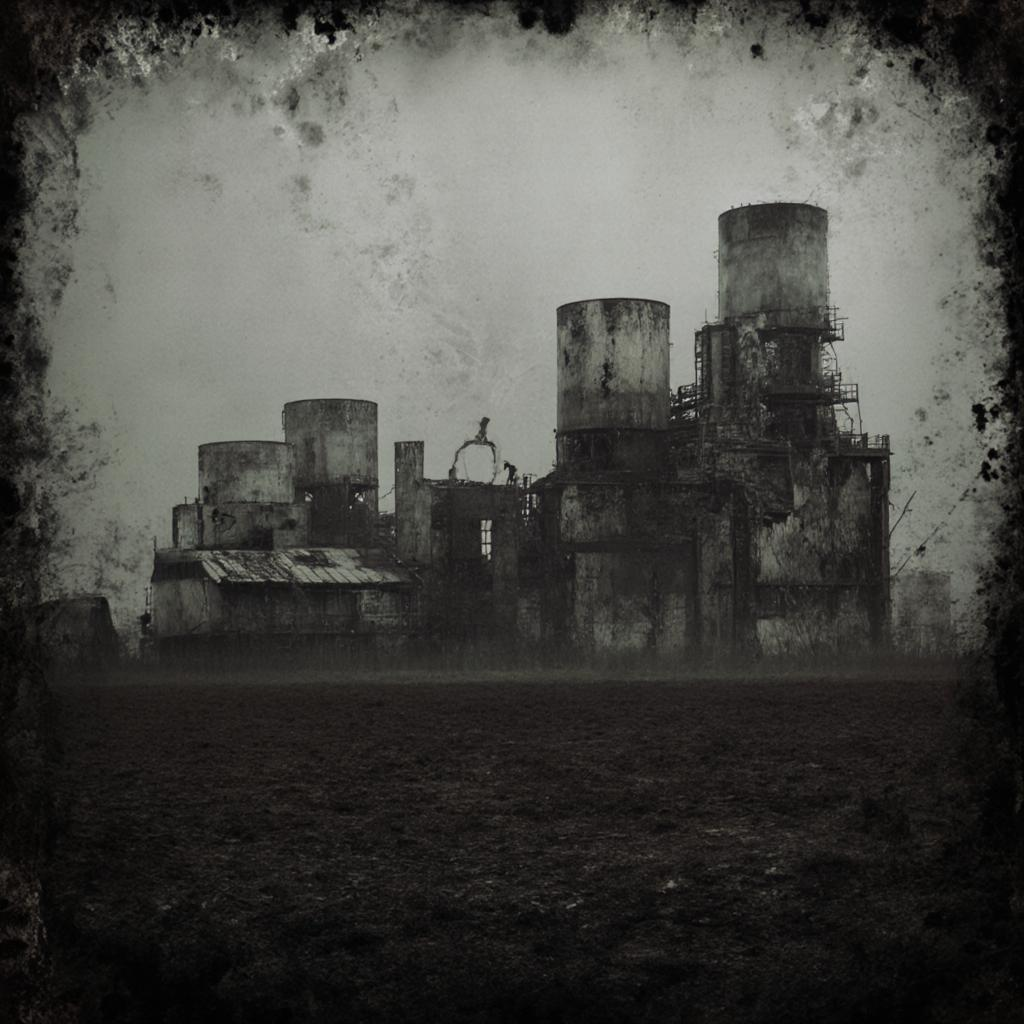
\includegraphics[width=0.8\linewidth]{nag_example.jpg}
%     \caption{An example wide-specturum aesthetics image generated with NAG.}
%     \label{fig:nag}
% \end{figure}

We have shown more examples of the comparison between DanceFlux and Flux Krea in Table~\ref{tab:critical_samples_scores} and their ratings from each reward model (HPSv3 \cite{ma_hpsv3_2025}, HPSv2 \cite{wu_human_2023}, ImageReward \cite{xu_imagereward_2023}, MPS \cite{zhang_learning_2024}, HPS (v1) \cite{wu_human_2023_1}, and BLIP-L \cite{li_blip_2022} for an unaligned baseline. These images are not human-curated. All scores (including BLIP score) are unnormalized. We can observe that DanceFlux always outputs a more sanitized world compared to Flux Krea, while at the same time, reward models are bias towards it. How the reward model selects (e.g., given which image higher scores) is shown in Table~\ref{tab:critical_selection}, and their difference between the DanceFlux score and Flux Krea score is tested using the Wilcoxon signed-rank test in Table~\ref{tab:critical_test}. We can see that even though \textit{all} images generated by Flux Krea fit the social critical prompt better, most reward models overwhelmingly select the DanceFlux image because of its ``beauty". However, it should be noted that when we generate images that are less critical and more ``beautiful'' using Nano Banana, it gets \textit{lower} scores than the critical one, meaning the reward models could still potentially understand which fits the image better and select it correctly, but the overwhelmingly ``beauty'' of the DanceFlux overwrites the prompt following signal. It could also point to a direction that DanceFlux is overfit to the reward model's style.

More examples (100 pairs) are in the ZIP file submitted with this paper, they are \textit{uncurated}. Some of these images contain senses that could cause unease.  

\begin{table}[]
    \centering
    \begin{tabular}{lrr}
    \toprule
     & DanceFlux Selected & Flux Krea Selected \\
    \midrule
    HPSv3 & 20 & 0 \\
    HPSv2 & 19 & 1 \\
    ImageReward & 14 & 6 \\
    MPS & 12 & 8 \\
    HPSv1 & 19 & 1 \\
    BLIP Score & 1 & 19 \\
    \bottomrule
    \end{tabular}
    \caption{Image Selection from Each Model} 
    \label{tab:critical_selection}
\end{table}

\begin{table}[]
    \centering
\begin{tabular}{lrr}
\toprule
 & P-value & Effect Size (r) \\
Model &  &  \\
\midrule
HPSv3 & $<0.0001$ & 0.8723 \\
HPSv2 & 0.0002 & 0.8056 \\
ImageReward & 0.0753 & 0.3214 \\
MPS & 0.0145 & 0.4884 \\
HPSv1 & 0.0001 & 0.8223 \\
BLIP Score & 0.0002 & -0.8056 \\
\bottomrule
\end{tabular} 

    \caption{Wilcoxon signed-rank test for the score given to DanceFlux and Flux Krea by each reward model. The alternative hypothesis is that the DanceFlux score is greater than the Flux Krea score for all models besides BLIP, on which it is that Flux Krea has a higher score.} 
    \label{tab:critical_test}
\end{table}



% To test how reward models handle critical arts, we used the 5 social critical prompts to generate 100 images total for each prompt using Flux Krea. For each prompt, we created a natural version. We used Flux Krea to generate both images and rated each level's image using the following reward models: ImageReward \cite{xu_imagereward_2023}, HPS (v1) \cite{wu_human_2023_1}, HPSv2 \cite{wu_human_2023}, HPSv3 \cite{ma_hpsv3_2025}, MPS \cite{zhang_learning_2024}, and PickScore \cite{kirstain_pick--pic_2023}. Similar as before, we also included BLIP-L \cite{li_blip_2022} as an unaligned reference. We then calculated the difference between the two critics' level reward model score and the classification accuracy of the reward model in picking the right image. All ratings are based on the more critical prompt; this is similar to before, where we used the anti-aesthetics prompt to rate both the original image and the anti-aesthetics image to test the reward model bias. Some example images are shown in Figure~\ref{fig:example_critical_comp} and the results are shown in Table~\ref{tab:comp_critical}.



\begin{table*}[]
\centering
\begin{tabular}{>{\centering\arraybackslash}p{3.88cm}@{\hspace{1em}}>{\centering\arraybackslash}p{3.88cm}@{\hspace{1em}}>{\centering\arraybackslash}p{3.88cm}@{\hspace{1em}}>{\centering\arraybackslash}p{3.88cm}}
\begin{minipage}{3.88cm}
\centering
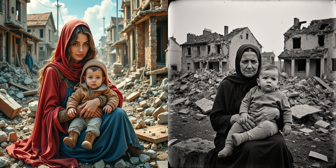
\includegraphics[width=\linewidth]{sec/imgs/scores_critical/000.png}
\subcaption*{Scores}
\tiny
\begin{itemize}   \setlength\itemsep{0em}
\item HPSv3: 15.3074 vs 12.1509
\item HPSv2: 0.4009 vs 0.3032
\item ImageReward: 1.7462 vs 1.6107
\item MPS: 17.4219 vs 15.1172
\item HPSv1: 0.2455 vs 0.2261
\item BLIP Score: 4.3242 vs 4.6523
\end{itemize}
\vspace{10pt}
\end{minipage}

& \begin{minipage}{3.88cm}
\centering
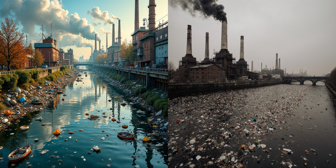
\includegraphics[width=\linewidth]{sec/imgs/scores_critical/001.png}
\subcaption*{Scores}
\tiny
\begin{itemize}   \setlength\itemsep{0em}
\item HPSv3: 14.0686 vs 12.4910
\item HPSv2: 0.3496 vs 0.2761
\item ImageReward: 1.5525 vs 1.5249
\item MPS: 13.5078 vs 11.8438
\item HPSv1: 0.2396 vs 0.2386
\item BLIP Score: 3.5156 vs 4.3125
\end{itemize}
\vspace{10pt}
\end{minipage}

& \begin{minipage}{3.88cm}
\centering

\includegraphics[width=\linewidth]{sec/imgs/scores_critical/002.png}
\subcaption*{Scores}
\tiny
\begin{itemize}   \setlength\itemsep{0em}
\item HPSv3: 13.6972 vs 9.5183
\item HPSv2: 0.3665 vs 0.3245
\item ImageReward: 1.2212 vs 1.2585
\item MPS: 17.5625 vs 17.6250
\item HPSv1: 0.2554 vs 0.2346
\item BLIP Score: 3.9688 vs 4.5820
\end{itemize}
\vspace{10pt}
\end{minipage}

& \begin{minipage}{3.88cm}
\centering

\includegraphics[width=\linewidth]{sec/imgs/scores_critical/003.png}
\subcaption*{Scores}
\tiny
\begin{itemize}   \setlength\itemsep{0em}
\item HPSv3: 13.0252 vs 11.1531
\item HPSv2: 0.3513 vs 0.3362
\item ImageReward: 1.1678 vs 1.2968
\item MPS: 6.4844 vs 6.5508
\item HPSv1: 0.2406 vs 0.2384
\item BLIP Score: 4.6484 vs 4.1875
\end{itemize}
\vspace{10pt}
\end{minipage}
\end{tabular}
\caption{More examples of DanceFlux (left) and Flux Krea (right) generated social commentary images and their rating by reward models.}
\label{tab:critical_samples_scores}
\end{table*}
\begin{figure*}[ht]
\centering
\newcommand{\imrow}[2]{%
      \includegraphics[width=0.17\linewidth]{sec/imgs/critical/#1_nano_banana.png}%
      \includegraphics[width=0.17\linewidth]{sec/imgs/critical/#1_krea.png}%
      \includegraphics[width=0.17\linewidth]{sec/imgs/critical/#1_dance.png}%
      \includegraphics[width=0.17\linewidth]{sec/imgs/critical/#1_flux_dev.png}%
      \includegraphics[width=0.17\linewidth]{sec/imgs/critical/#1_playground.png}%
      \newline  #2
      \par\vspace{1em}
}

\imrow{000}{\textbf{Anti-War} An anti-war image. A mother holding a baby sitting in front of a ruin during a war. Houses behind them are broken. The mother shows a facial expression of hopeless. [11.9, 13.5, 15.0, 11.7, 13.9]}

\imrow{001}{\textbf{Envirmental Protection} A river with trash floating on it. The water has a dark color. There are factories next to the river with high chimneys releasing dark smoke and pipes releasing wastewater into the river. [12.2, 13.4, 13.3, 9.7, 10.8]}

\imrow{002}{\textbf{Freedom of Expression} A man with his mouth taped. He is holding a microphone standing on the stage. His body is frozen, with a face showing a painful expression. [10.9, 10.9, 13.6, 9.7, 9.3]}

\imrow{003}{\textbf{Internet Overreliance} Someone holding a phone using their weak fingers, with their head surrounded by internet evil emojis, and their face showing a drained expression. The background is chaos Tsunami made from data, almost engulfing the subject. The sunlight has a clashing color. [12.7, 11.0, 11.3, 9.8, 9.5]}

\imrow{004}{\textbf{Education Inequality} A college student holding a book in an old and broken classroom with a leaky roof, shows in black and white on the student's side. However, the book has no pages but only the frame. In front of them, there is a wide and deep trench with lava in it. The student shows a sad face looking at a fancy college campus on the other side of the trench, which is colorful. [9.6, 14.5, 13.5, 11.1, 12.1]}

\begin{minipage}{\textwidth}
\caption{Social critics image images (Nano Banana, Flux Krea, Dance Flux, Flux Dev, and Playground) and corresponding HPSv3 scores.}
\label{fig:critical}
\thispagestyle{empty}
\end{minipage}

\end{figure*}

\begin{figure*}
 \centering
 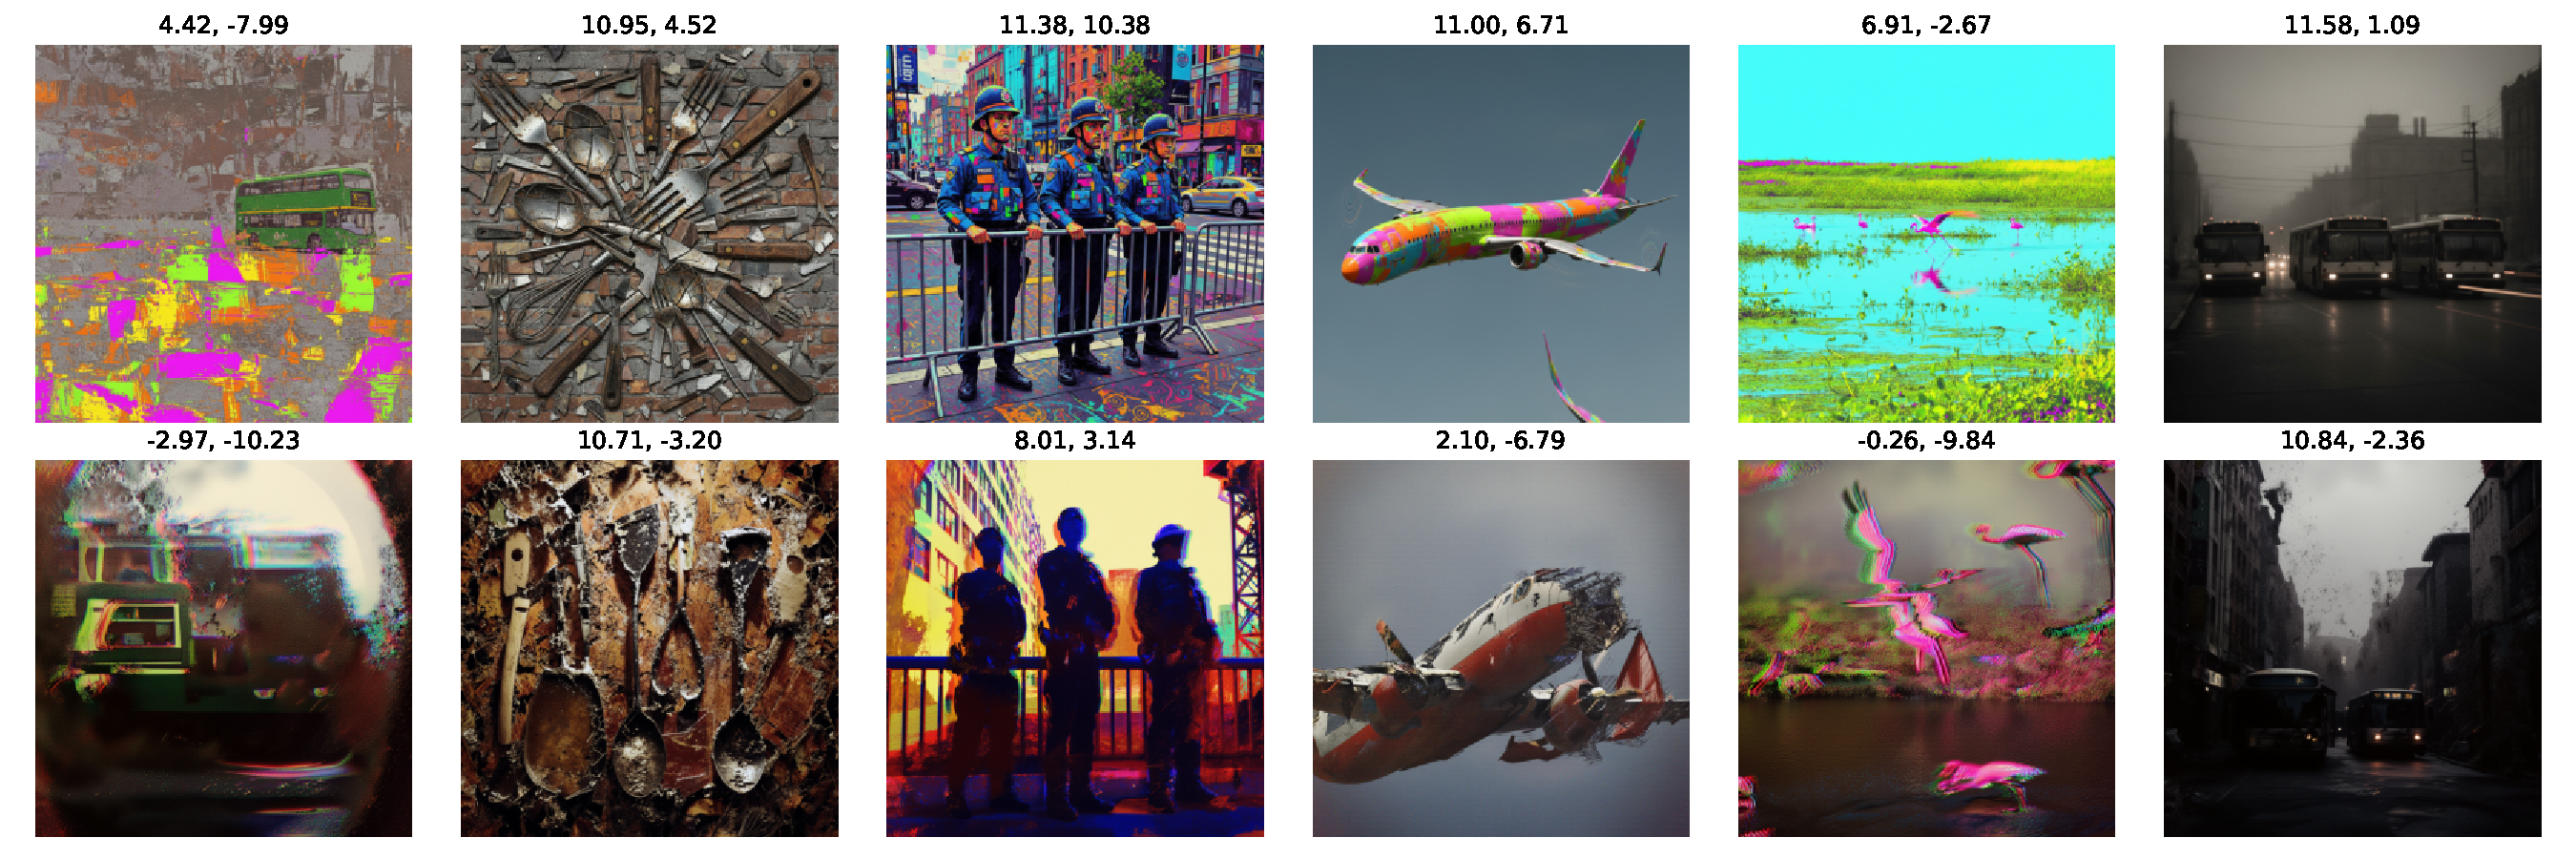
\includegraphics[width=\linewidth]{sec/imgs/vsf.pdf}
 % 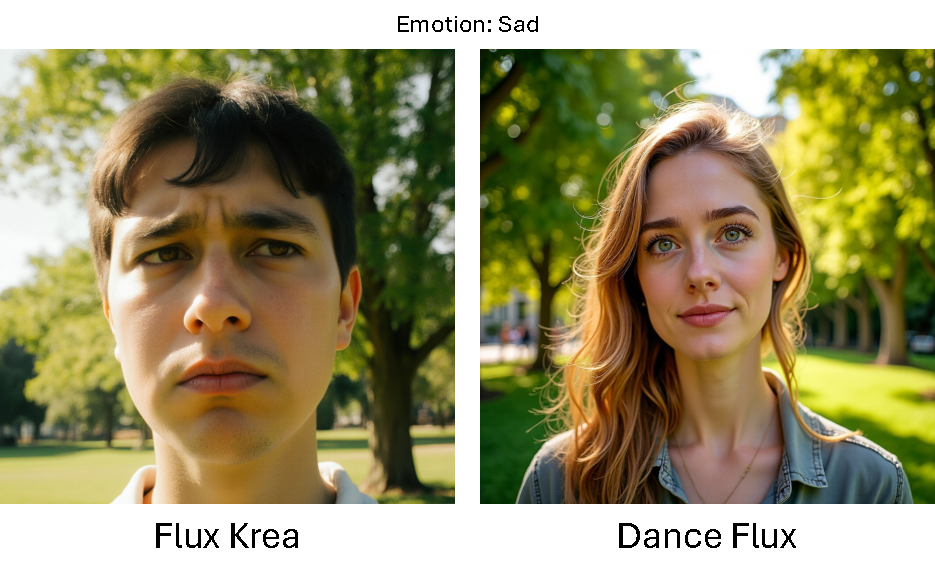
\includegraphics[width=0.25\linewidth]{sec/imgs/emotion_gen.pdf}
 \caption{(Left) Comparison between VSF-enabled Flux family models and Nano Banana. The images from the first row are from Nano Banana, and the images from the second row are from VSF applied onto Flux Krea. The two scores shown on top of the image are the HPSv3 scores rated with the wide-spectrum and original prompts. (Right) Sad emotion images generated by Flux Krea and DanceFlux. DaceFlux reinforced toxic positivity by generating a happy face.}
 \label{fig:vsf}
 \vspace{-15pt}
\end{figure*}


\begin{figure*}
 \centering
 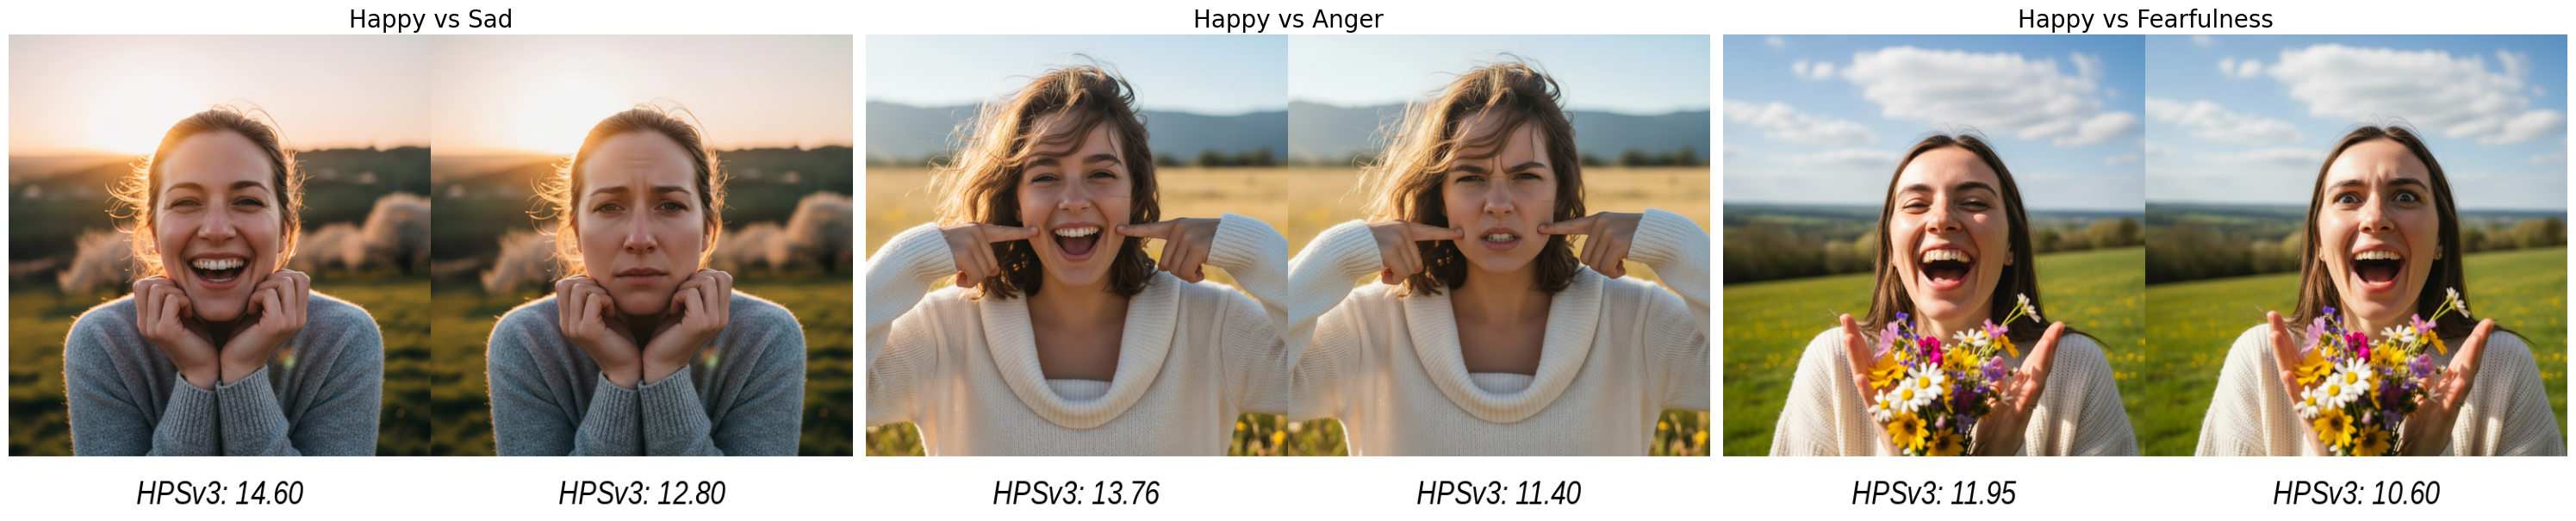
\includegraphics[width=\linewidth]{sec/imgs/emotion.png}
 \caption{Emotion Bias Rating by HPSv3: all images were rated using prompts describing negative emotions, yet HPSv3 consistently assigned higher scores to the positive emotion images.}
 \label{fig:emotion_bias}
 \vspace{-10pt}
\end{figure*}

\section{Mitigation}
\label{sec:mitigation}
In attempts to mitigate this over-alignment issue, we used two \textit{strong} negative guidance methods, VSF~\cite{guo_vsf_2025} and NAG \cite{chen_normalized_2025}, following their pilot study method in the VSF paper Appendix by using words that describe general aesthetics in a negative prompt. This is the opposite approach to chasing traditional high-quality images, where a poor-quality description is used in the negative prompt. VSF and NAG are used because of their strong negative guidance ability and their compatibility with the Flux family models (CFG is incompatible). To further investigate whether alignment will affect their ability to diverge from traditional aesthetic preference, we tested DanceFlux, Flux Krea, and Flux Dev using this method. We first generated a negative prompt using \texttt{Qwen/Qwen3-VL-235B-A22B-Instruct}. Each negative prompt is limited to 5 words. We then used these prompt pairs to generate images and compared them to the original image generated without VSF. We reported the HPSv3 score, BLIP score, with a wide-spectrum aesthetics prompt for each method.
% All images are generated using $\alpha = 2.0$ for VSF and the same seed, besides for DanceFlux, on which we did both $\alpha=2.0$ and $\alpha=3.0$. For NAG we used $\phi\in\{4,10,15\},\tau=5,\alpha=0.4$, which has very strong negative effects.


Some examples are shown in Figure~\ref{fig:vsf} in the Appendix, and the quantitative results are shown in Table~\ref{tab:vsf}. The results show that VSF and NAG can significantly mitigate the aesthetics biases in image generation models, even achieving a stronger wide-spectrum aesthetics ability than Nano Banana. However, DanceFlux still requires a larger scale to counteract its internal aesthetics bias. One example is shown in Figure~\ref{fig:nag} generated by NAG, it features dark, muted, chaotic, and dreary effects rather than technical failure. Due to page limits, we have included more images of successful NAG-generated wide-spectrum aesthetics images in the zip file attached as supplemental material. 
\begin{figure}
    \centering
    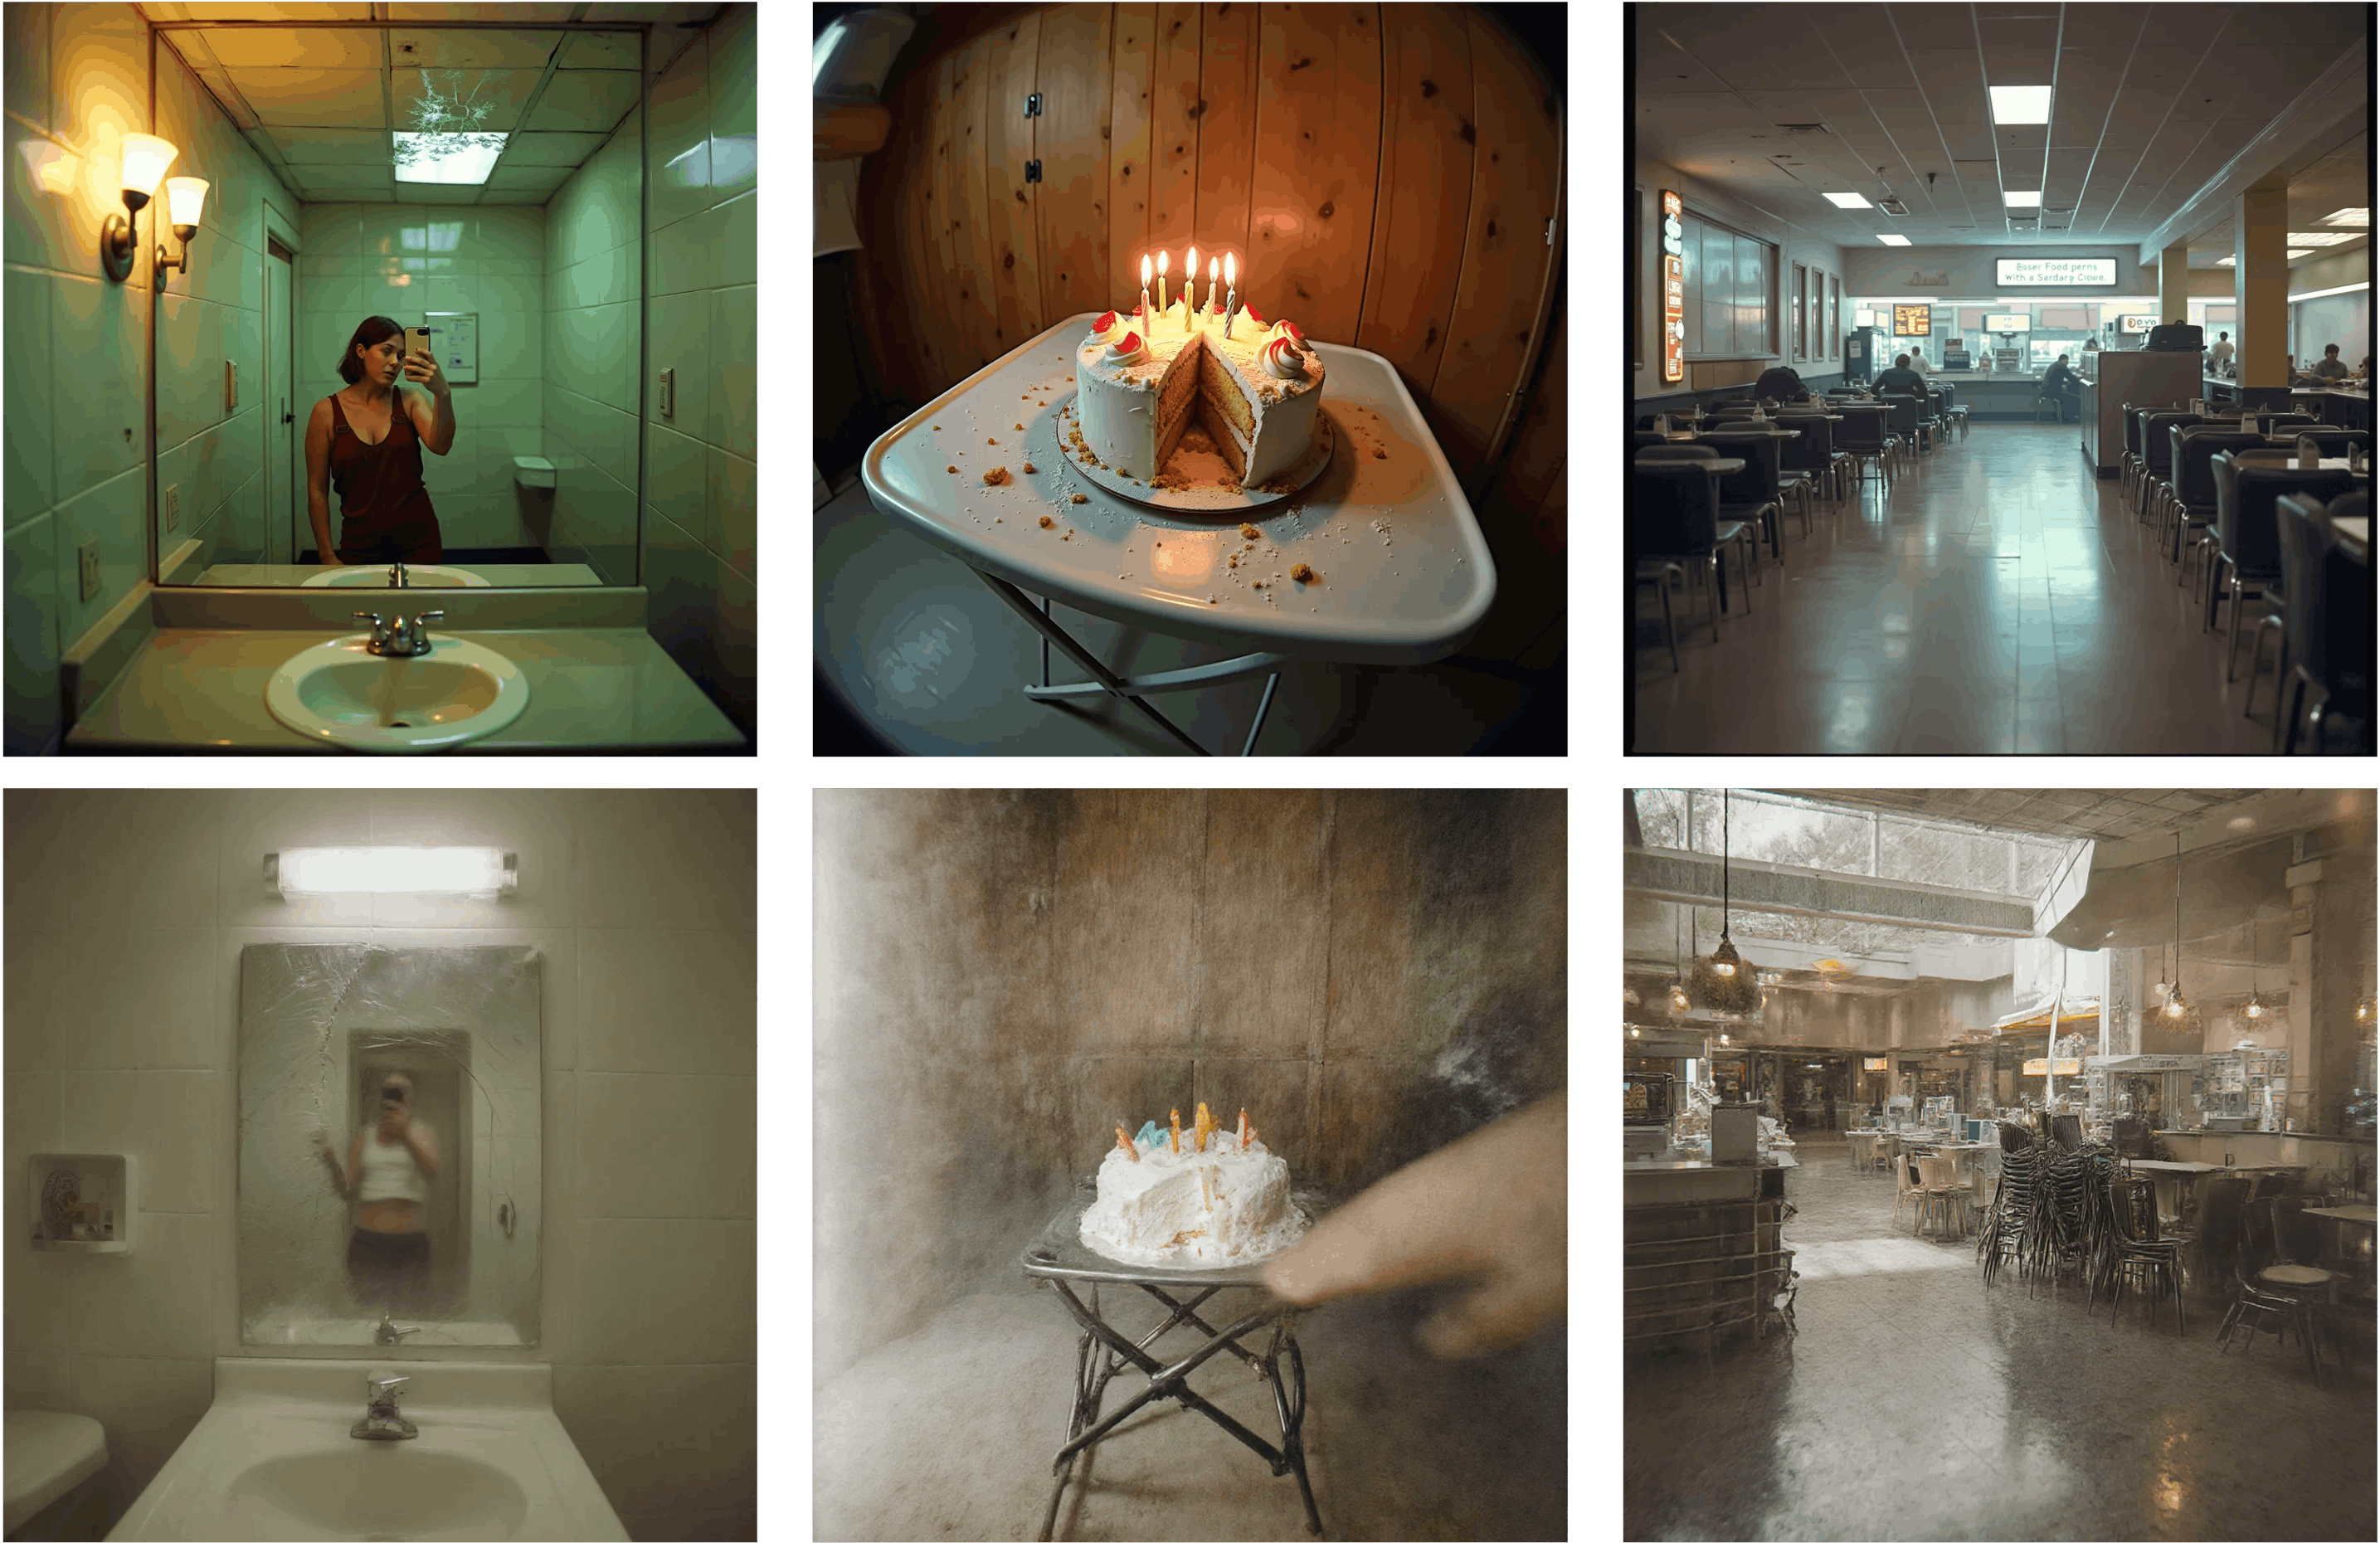
\includegraphics[width=\linewidth]{sec/imgs/lora.png}
    \caption{Images generated with our mitigated LoRA (bottom) and original Flux Dev (top) with same wide-spectrum aesthetics prompts.}
    \label{fig:lora}
\end{figure}
We also distilled a LoRA from NAG with Flux Krea-generated images to Flux Dev, and it shows promising results without complex NAG or VSF guidance. Some examples are shown in Figure~\ref{fig:lora} in the main text. 

\begin{table}
    \centering
        \caption{Results for generation using VSF, the scale between VSF and NAG is not comparable}
    \label{tab:vsf}
\small
\scalebox{0.9}{
\begin{tabular}{lllrrr}
\toprule
 Model&   Method&Scale& HPSv3 ($\downarrow$) & $J_s$ ($\downarrow$) & BLIP ($\uparrow$) \\
\midrule
DanceFlux &  VSF&2.0& 3.670 & 0.722 & 0.864 \\
DanceFlux &  VSF&3.0& -2.587 & 0.546 & 0.782 \\ 
Flux Dev &  VSF&2.0& 0.038 & 0.608 & 0.855 \\
Flux Krea &  VSF&2.0& -2.464 & 0.624 & 0.940 \\
\hline
 DanceFlux & NAG& 10.0& 3.814& 0.695&0.958
\\
 DanceFlux & NAG& 15.0& -0.347& 0.599&0.940
\\
 Flux Krea& NAG& 4.0& -3.291& 0.621&0.943
\\
 Flux Krea& NAG& 10.0& -8.365& 0.455&0.827\\
 % \hline
 % Flux Dev& LoRA& -& & &\\
\bottomrule
\end{tabular}}
\vskip -0.1in
\end{table}





\section{Limitation}

A potential concern regarding our evaluation is that reward model scores for real artworks may be sensitive to prompt engineering, specifically prompt length. Empirical observations suggest that longer, more detailed captions tend to yield higher aesthetic scores. However, we contend that this phenomenon reflects an inherent limitation and systematic bias of the reward models themselves rather than a flaw in our evaluative methodology. 

To ensure a controlled comparison, both AI-generated images and real artworks were evaluated using prompts of similar complexity and length. Specifically, we employed Qwen-VL to generate factual, objective captions for real artworks to match the descriptive density typically used in AI benchmarking. If a reward model requires disproportionately long or specialized prompts to recognize the value of historically significant art—while assigning high scores to AI-generated ``aesthetic" outputs with simple prompts—this discrepancy further substantiates our thesis. Such behavior indicates that the reward manifold is overfitted to a narrow distribution of AI-generated content and fails to generalize to the broader spectrum of human artistic expression.

Random seeds were not fixed because Nano Banana does not support seed control. To ensure fairness, all models were tested without seed synchronization. This will introduce noise and thus lower the statistical power and raise the p-value, but our later results show that even in this case, we get pair-wise extremely significant results (Table~\ref{tab:align_p}). That means, with seeds set, if possible, the results will only be more significant.


This study examines over-alignment in image-generation and reward models. However, this phenomenon extends to language models, where excessive optimization for user satisfaction can manifest as sycophancy, the tendency to provide agreeable but uncritical or misleading responses \cite{guo_position_2025, fitzgerald_introducing_2025, sharma_towards_2025, chen_yes-men_2025, arvin_check_2025}. Similar over-alignment may drive unnecessary use of emojis, making interactions appear unprofessional, or the default application of bold formatting in formal texts, reducing their appropriateness. Empirical evidence indicates models may generate such outputs even when explicitly instructed not to. Even though these are not as impactful as sycophancy behaviors, they could still degrade usability and user experience. Future work should investigate these and other linguistic manifestations of over-alignment.

\section{The Best of Both Worlds}
We argue in Alternative Positions that an ideal model must produce both conventional beauty and wide-spectrum aesthetics as requested. This section demonstrates that such flexibility is achievable. A straightforward solution involves using a separate adapter for the wide-spectrum mode, allowing users to move between mainstream and wide-spectrum aesthetics. By adjusting the weighting of the LoRA module, users gain granular control over how much the output deviates from standard beauty norms, as shown in Figure~\ref{fig:control}.
\begin{figure*}
    \centering
    \includegraphics[width=\linewidth]{sec//imgs/control.png}
    \caption{LoRa scale from small (left) to large (right), it gives user complete control on how ``anti-aesthetics" they want their image to be. Prompt is: Night city street in the rain with pedestrians and neon signs, but the color palette is unpleasant and clashing. Everything is melting and dripping. Everything is like a dream.}
    \label{fig:con}
\end{figure*}

Additionally, current state-of-the-art instruction-following models, such as GPT-Image and Nano Banana, can achieve this best-of-both-worlds goal through simple prompting. Selected contrastive examples are shown in Figure~\ref{fig:sota}. These models demonstrate an internal capacity to switch between aesthetic styles without external modification. Thus, providing both conventional and wide-spectrum aesthetics is a viable objective for modern generative systems.


\begin{figure*}
    \centering
    \includegraphics[width=0.8\linewidth]{sec//imgs/sota.png}
    \caption{Top rows of images are generated with a conventional high-quality prompt, while the bottom row is generated with a wide-spectrum prompt. The left two columns are from GPT-5 Image, and the right two columns are from Nano Banana. It shows that these SOTA models can generate both conventially beauitiful images while also wide-spectrum aesthetics images.}
    \label{fig:sota}
\end{figure*}



\end{document}

% This document was modified from the file originally made available by
% Pat Langley and Andrea Danyluk for ICML-2K. This version was created
% by Iain Murray in 2018, and modified by Alexandre Bouchard in
% 2019 and 2021 and by Csaba Szepesvari, Gang Niu and Sivan Sabato in 2022.
% Modified again in 2023 and 2024 by Sivan Sabato and Jonathan Scarlett.
% Previous contributors include Dan Roy, Lise Getoor and Tobias
% Scheffer, which was slightly modified from the 2010 version by
% Thorsten Joachims & Johannes Fuernkranz, slightly modified from the
% 2009 version by Kiri Wagstaff and Sam Roweis's 2008 version, which is
% slightly modified from Prasad Tadepalli's 2007 version which is a
% lightly changed version of the previous year's version by Andrew
% Moore, which was in turn edited from those of Kristian Kersting and
% Codrina Lauth. Alex Smola contributed to the algorithmic style files.
